\documentclass[twoside]{article}
\usepackage[utf8]{inputenc}
\usepackage[T1]{fontenc}
\usepackage[frenchb]{babel}

\usepackage{a4wide}
\usepackage{graphicx}
\graphicspath{{images/}}
%\usepackage{subfig}
\usepackage{tikz}
\usetikzlibrary{shapes,arrows}
\usepackage{pgfplots}
\pgfplotsset{compat=newest}
\pgfplotsset{plot coordinates/math parser=false}
\newlength\figureheight
\newlength\figurewidth
\pgfkeys{/pgf/number format/.cd, set decimal separator={,\!}, 1000 sep={\,},}
\usepackage{ifthen}
\usepackage{ifpdf}
\ifpdf
\usepackage[pdftex]{hyperref}
\else
\usepackage{hyperref}
\fi
\usepackage{color}
\hypersetup{%
colorlinks=true,
linkcolor=black,
citecolor=black,
urlcolor=black}

\renewcommand{\baselinestretch}{1.05}
\usepackage{fancyhdr}
\pagestyle{fancy}
\fancyfoot{}
\fancyhead[LE,RO]{\bfseries\thepage}
\fancyhead[RE]{\bfseries\nouppercase{\leftmark}}
\fancyhead[LO]{\bfseries\nouppercase{\rightmark}}
\setlength{\headheight}{15pt}

\let\headruleORIG\headrule
\renewcommand{\headrule}{\color{black} \headruleORIG}
\renewcommand{\headrulewidth}{1.0pt}
\usepackage{colortbl}
\arrayrulecolor{black}

\fancypagestyle{plain}{
  \fancyhead{}
  \fancyfoot[C]{\thepage}
  \renewcommand{\headrulewidth}{0pt}
}

\makeatletter
\def\@textbottom{\vskip \z@ \@plus 1pt}
\let\@texttop\relax
\makeatother

\makeatletter
\def\cleardoublepage{\clearpage\if@twoside \ifodd\c@page\else%
  \hbox{}%
  \thispagestyle{empty}%
  \newpage%
  \if@twocolumn\hbox{}\newpage\fi\fi\fi}
\makeatother

\usepackage{amsthm}
\usepackage{amssymb,amsmath,bbm}
\usepackage{array}
\usepackage{bm}
\usepackage{multirow}
\usepackage[footnote]{acronym}

\newtheoremstyle{break}
  {11pt}{11pt}%
  {\itshape}{}%
  {\bfseries}{}%
  {\newline}{}%
\theoremstyle{break}

\parskip=5pt
% ============== HEADER INITIAL ==============
% === AJOUTER LES MODIFICATIONS EN DESSOUS ===

\renewcommand{\thesection}{\Roman{section}}
\renewcommand{\thesubsection}{\arabic{subsection}}
\usepackage{enumitem}
\setlist[itemize]{label=\textbullet}
\usepackage{subcaption}


\begin{document}

\begin{titlepage}\begin{center}

    
\includegraphics[width=0.6\textwidth]{images/logo-isae-supaero.png}\\[1cm]

    {\large Projet Ingénierie et Entrepreneuriat}\\[0.5cm]

    \rule{\linewidth}{0.5mm}\\[0.4cm]
    {\huge \bfseries Analyse de schémas numériques d'intégration temporelle\\[0.4cm]}
    \rule{\linewidth}{0.5mm}\\[1.5cm]

    \noindent
    \begin{minipage}{0.4\textwidth}\begin{flushleft}\large
        \emph{Auteurs :}\\
        Sara \textsc{Barassa-Ramos}\\
        Jean-Baptiste \textsc{Fourtout}\\
        Théo \textsc{Maes} \\
        Louis \textsc{Reboul}\\
        Pierre \textsc{Seize}\\
    \end{flushleft}\end{minipage}%
    \begin{minipage}{0.4\textwidth}\begin{flushright}\large
        \emph{Encadrants :}\\
        Xavier \textsc{Vasseur}\\
        Guillaume \textsc{Puigt}\\
        Rémi \textsc{LeBouteiller}
    \end{flushright}\end{minipage}

    \vfill
    \today

\end{center}\end{titlepage}


\textbf{Résumé ---} L'intérêt du client se porte sur les méthodes de modélisation numériques des phénomènes physiques liés à la mécanique des fluides.

Les phénomènes concernés sont modélisés à l'aide d'équations aux dérivées partielles. Obtenir des solutions de celles-ci nécessite de résoudre à la fois un problème spatial et un problème temporel. Ce qui limite aujourd'hui les performances des codes de calcul est leur capacité à résoudre la partie temporelle du problème.

L'enjeu de ce projet était donc d'estimer le potentiel d'un nouveau type de méthodes temporelles, appelées méthodes exponentielles. Nous avons pu montrer qu'il y a un réel bénéfice à utiliser ces méthodes par rapport aux méthodes classiques sur certains types de problèmes. Pour d'autres types de problèmes, comme l'équation de Burgers, nous avons pu montrer que ces méthodes fournissent un résultat correct sans pouvoir conclure sur leurs performances réelles.

Ces méthodes nécessitent le calcul d'exponentielles de matrices pour fonctionner. Ce calcul étant lourd lorsque lesdites matrices sont de dimension conséquente, il est nécessaire d'utiliser des méthodes spécifiques pour accélérer les processus de calcul. Nous avons pu montrer qu'il était possible de réaliser un gain de temps substantiel en utilisant des méthodes basées sur les espaces de Krylov.

\textbf{Déclaration d'authenticité ---} Nous déclarons avoir personnellement réalisé ce projet, rédigé les différents documents et attestons également ne pas avoir eu recours au plagiat et avoir consciencieusement mentionné tout emprunt fait à autrui.


\noindent\rule[2pt]{\textwidth}{0.5pt}
\part*{Introduction}

\paragraph{}
Ce document est rédigé dans le cadre du Projet Ingénierie et Entrepreneuriat en dernière année de l'ISAE SUPAERO, en partenariat avec l'ONERA. Il s'agit ici d'analyser les performances de schémas numériques d’intégration temporelle pour la résolution de problèmes du type advection-diffusion rencontrés en mécanique des fluides. La particularité des problèmes de mécanique des fluides c'est que les équations qui régissent la physique sont des équations différentielles partielles. Ce qui implique qu'il faut savoir résoudre des équations à la fois en temps et en espace. Aujourd'hui de nombreuses recherches sur les méthodes de résolution spatiales ont permis d'obtenir des résultats très prometteurs. Mais peu de progrès ont été fait sur la résolution temporelle. C'est donc l'objet de ce projet.

\paragraph{}
En effet l'objectif est d'implémenter des méthodes numériques d'intégration temporelles dites \og exponentielles \fg{} d'ordre plus élevés que celles utilisées usuellement. Ces méthodes permettraient d'augmenter le pas de temps d'un calcul CFD. Ce qui réellement permet à un industriel de réaliser des simulations numériques bien plus rapides qu'avec une méthode usuelle. Par conséquent ces méthodes semblent très intéressantes pour réduire les coûts de calcul. Néanmoins ces méthodes n'intéresseront pas notre client si elles ne fonctionnent pas avec les méthodes spatiales. Le couplage des deux méthodes est donc le deuxième enjeu primordial de ce projet.

\paragraph{}
Le travail effectué se base donc sur la publication de papiers scientifiques. Afin de valider au fur et à mesure le travail effectué nous testerons nos méthodes sur des cas simples que nous complexifierons avec l'avancée du travail. Nous réaliserons la programmation avec le langage Python qui est un langage open source et choisit par le client.


\clearpage

\tableofcontents
\clearpage

\section{Gestion de projet}

\paragraph{}
Cette partie consiste à exposer la manière dont nous nous sommes organisés pour la réalisation de ce projet. Ce sujet de PIE s'inscrit globalement dans une stratégie commune de recherche entre l'ISAE-SUPAERO et l'ONERA. L'objectif est l'amélioration du code de calcul JAGUAR basé sur les différences spectrales ayant pour objectif d'effectuer des simulations numériques LES pour des applications CFD.

\paragraph{}
Les méthodes spectrales discontinues consistent à représenter la solution par cellule de calcul sur une base polynômiale et à prendre en compte la discontinuité de la solution entre cellules par résolution d'un problème de Riemann. Assez récentes en CFD, leurs applications pour la LES est un sujet de recherche actuel. Aujourd'hui, les études se focalisent essentiellement sur la précision des schémas spatiaux pour la convection et la diffusion. Ici, on souhaite focaliser notre attention sur les schémas numériques d'intégration temporelle des équations dans un code prototype 1D. Après une analyse bibliographique sur les méthodes temporelles, nous proposons l'implémentation de plusieurs familles de schémas dans une maquette 1D puis de comparer les performances.

\subsection{Description du projet}

    \subsubsection{Objectifs du projet et résultats attendus}
        \paragraph{}
        Une première liste des objectifs attendus par le client est énumérée ci-après :
        \begin{itemize}
            \item une analyse bibliographique des différentes classes de méthodes
            \item une analyse approfondie des schémas numériques (précision, coût algorithmique, CFL max) 
            \item une maquette dans laquelle les schémas sont implémentés et plusieurs cas tests de validation 
            \item un rapport sur la comparaison croisée des schémas numériques
            \item une liste de recommandations du groupe sur le(s) meilleur(s) schéma(s)
        \end{itemize}

        \paragraph{}
        Afin de répondre au cahier des charges client nous devons implémenter les méthodes numériques en langage Python. Sur les conseils de notre client nous avons utilisé la plateforme de travail GitHub qui est très adaptée, pour travailler sur des fichiers de code informatique notamment. Ceci nous permet aussi d'avoir plusieurs sauvegardes de notre travail et cela prévient donc d'une éventuelle perte du code informatique.

        \paragraph{}
        La documentation détaillée du code est une requête du client c'est pourquoi nous avons utilisé le logiciel libre Sphinx pour créer la documentation du code. Ce programme, simple d'utilisation, permet de compiler une documentation au format \emph{html}, constituée de pages détaillées, comportant des fonctionnalités de navigation par lien hypertexte.

    \subsubsection{Les parties prenantes du projet}
        \paragraph{}
        Il est important de bien connaître toutes les parties prenantes du projet afin que la communication entre ces différentes parties soit fluide et efficace.
        \begin{itemize}
            \item Louis Reboul, Pierre Seize, Sara Barrasa-Ramos, Jean-Baptiste Fourtout et Théo Maes : groupe d'étudiants de L'ISAE qui représente l'équipe de développeurs
            \item Guillaume Puigt : Client et encadrant technique de l'ONERA
            \item Xavier Vasseur : Client, encadrant technique et référent école
            \item Rémi Lebouteiller : Tuteur en gestion de projet
        \end{itemize}

        \paragraph{}
        Dans le but de garantir une bonne communication avec les différentes parties nous avons mis en place plusieurs interfaces de communication. Néanmoins nous les détaillerons un peu plus loin dans ce rapport.

    \subsubsection{Les contraintes identifiées}
        \paragraph{}
        Les contraintes connues portent sur l'environnement de développement du code informatique, elles sont imposées par le client :
        \begin{itemize}
            \item utilisation du langage de programmation Python, version 2.7
            \item Utilisation de la plateforme GitHub pour la gestion du versionnage des fichiers
        \end{itemize}

    \subsubsection{Hypothèses de travail}
        \paragraph{}
        Les hypothèses du projet portent sur les ressources disponibles et la capacité de travail des membres de l'équipe de développement.
        \begin{itemize}
            \item L'équipe de développement peut fournir 4h à 8h de travail par semaine et par personne.
            \item La bibliographie est fournie par Guillaume Puigt et par Xavier Vasseur.
            \item Les algorithmes d'intégration spatiales sont fournis par Guillaume Puigt.
        \end{itemize}

        \paragraph{}
        Ayant identifié tous les objectifs et les contraintes associées, il nous faut établir une stratégie afin de se répartir la charge de travail de façon équivalente au sein de l'équipe.


\subsection{Organisation}

    \subsubsection{Outils de gestion de projet}
        \paragraph{}
        Les outils qui nous ont été très utiles pour mettre des limites à notre projet et de répartir les différentes tâches au sein de l'équipe sont principalement les diagrammes PBS et WBS.

        \paragraph{}
        Le diagramme PBS (Product Breakdown Structure) nous permet de savoir dans quelle ordre nous allons effectuer les différentes opérations pour aboutir à l'objectif du projet (figure \ref{PBS}).
        \begin{figure}
            \centering
            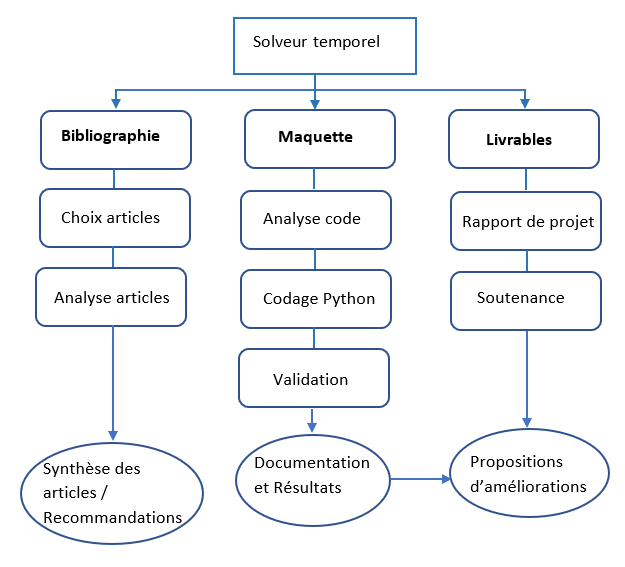
\includegraphics[width=0.6\textwidth]{images/pbs.png}
            \caption{Diagramme PBS}
            \label{PBS}
        \end{figure}

        \paragraph{}
        D'un autre côté, le diagramme WBS (Working Breakdown Structure) nous indique plutôt comment nous allons effectuer ces opérations. Cela permet de définir différentes tâches et nous répartir le travail de manière équitable pour lisser la charge de travail sur chacun des membres de l'équipe (figure \ref{WBS}).
        \begin{figure}
            \centering
            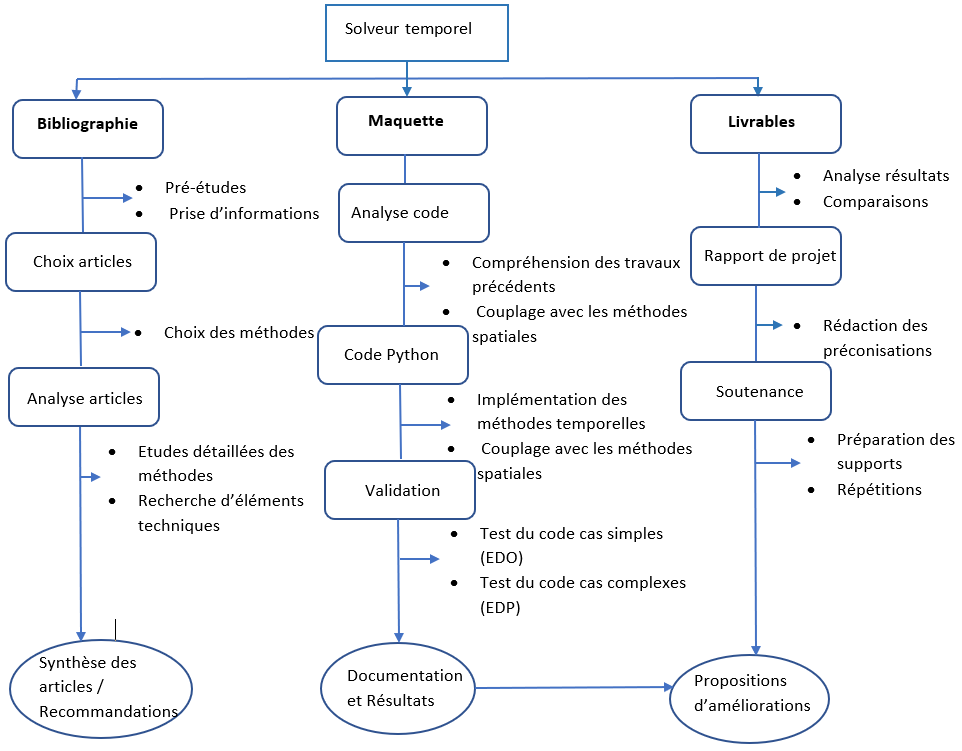
\includegraphics[width=0.8\textwidth]{images/wbs.png}
            \caption{Diagramme WBS}
            \label{WBS}
        \end{figure}

        \paragraph{}
        L'utilisation de ces outils nous a permis de délimiter le périmètre de travail afin de rester focalisé sur l'objectif du client et de ne pas divaguer. Ici le diagramme WBS (figure \ref{WBS}) n'est pas détaillé à son maximum par soucis de lisibilité. Cet outil donne une bonne idée d'ensemble de toutes les tâches qui sont à réaliser dans un ordre précis pour aboutir au résultat final du projet. 

    \subsubsection{Organisation de l'équipe}
        \paragraph{}
        La répartition du travail s'est faite assez naturellement en deux équipes grâce aux diagrammes PBS et WBS vu précédemment. Nous connaissions très bien les limites de notre projet et les étapes à effectuer pour parvenir aux objectifs du client. Chacun a pu trouver sa place au sein de la configuration suivante (figure \ref{fig:OBS}):
        \begin{itemize}
            \item Théo Maes est le chef de projet.
            \item L'équipe développement, coordonnée par Sara Barrasa-Ramos, sera responsable de l'implémentation des méthodes numériques. Elle sera composée de :
            \begin{itemize}
                \item Louis Reboul,
                \item Sara Barrasa-Ramos,
                \item Théo Maes.
            \end{itemize}
            \item L'équipe couplage, coordonnée par Pierre Seize, sera responsable de rendre compatible les schémas numériques d'intégration temporelle avec les schémas numériques d'intégration spatiale existants. Elle sera composée de :
            \begin{itemize}
                \item Pierre Seize,
                \item Jean-Baptiste Fourtout.
            \end{itemize}
        \end{itemize}
        \begin{figure}
            \centering
            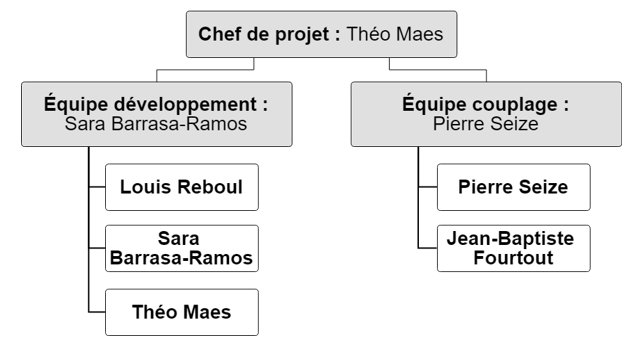
\includegraphics[scale=0.7]{images/obs.png}
            \caption{Organisation de l'équipe} 
            \label{fig:OBS}
        \end{figure}

        \paragraph{}
        Cette répartition ayant été faite en consensus avec l'ensemble de l'équipe, en prenant en compte les préférences de chacun et le niveau de connaissance dans ce domaine d'application des sciences. Nous nous sommes efforcés de conserver le plus possible cette répartition du travail. Néanmoins nous avons été contraints d'effectuer certains changements temporaires de ressources humaines au cours du projet pour pallier des problématiques qui seront expliquées plus en détail par la suite.

    \subsubsection{Organisation du travail}
        \paragraph{}
        Il nous semble important d'aborder la matrice RACI qui est née de l'association des diagrammes OBS et WBS. En effet, cette matrice permet de repérer le rôle de chacun des membres de l'équipe pour une tâche donnée comme il est indiqué figure \ref{fig:RACI}.

        \paragraph{}
        La lettre R signifie "Réalisation", dans le sens où les personnes assujetties à cette lettre pour une tâche doivent fournir un travail. C'est différent si la personne est associée à la lettre C, signifiant "Consultation", car cela signifie simplement qu'elle peut posséder des connaissances, un point de vue intéressant sur la réalisation de la tâche. Cette consultation est effectuée en amont de la réalisation. L'indice I pour "Information" concerne les conseils promulgués par des gens qui ont la connaissance pour améliorer la réalisation de la tâche. Et enfin la lettre A signifie "Approbation" et concerne les personnes qui vont prendre les décisions. Dans le cadre de notre projet, cela se restreint au chef d'équipe en charge de la tache en question.
        \begin{figure}
            \centering
            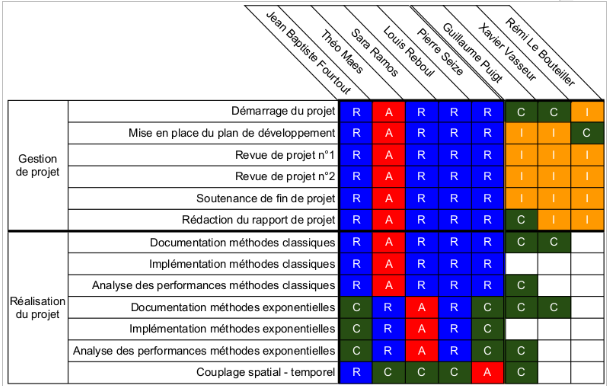
\includegraphics[width=\textwidth]{images/raci.png}
            \caption{Matrice RACI} 
            \label{fig:RACI}
        \end{figure}

        \paragraph{}
        Il est naturel que le chef de projet ne sert pas qu'à l'approbation des tâches réalisées par ses camarades, il participe au même titre que tout le monde.

        \paragraph{}
        Cette matrice est intéressante car elle permet à chacun des collaborateurs de voir avec qui il travaille sur une même tâche et de pouvoir échanger avec eux. On identifie d'autant plus rapidement les personnes "expertes" qui sauront nous orienter dans le cas d'un blocage lors de la réalisation d'une tâche.


\subsection{Processus du développement}

    \subsubsection{Logique de développement}
        \paragraph{}
        Notre logique de développement du projet s'articule principalement sur les différents groupes de tâches qui ont été répertoriés dès la mise en place du projet à l'aide des diagrammes PBS et WBS.

        \paragraph{}
        En toute logique nous avons commencé par prendre connaissance de la bibliographie qui est directement fournie par notre client. Puis il a fallu prendre en main la programmation avec le langage Python car tous les développeurs n'avaient pas la même connaissance de ce langage informatique.

        \paragraph{}
        Une analyse approfondie des articles scientifiques et des recherches personnelles du groupe ont permis à l'équipe développement de faire un choix sur les méthodes temporelles qui seront étudiées plus en profondeur. C'est sur des conseils et en accord avec notre client que nous avons fait ces choix. En parallèle l'équipe se chargeant du couplage spatial-temporel devait comprendre en profondeur le fonctionnement du code informatique fournit pour établir une stratégie pour pouvoir y adapter le travail de l'équipe développement.

        \paragraph{}
        Ensuite, nous avons implémenté les nouvelles méthodes de résolution temporelle dites "Exponentielles", pendant que l'équipe couplage testait le couplage spatial-temporel avec les méthodes usuelles que l'équipe développement a mis très rapidement en oeuvre au début du projet.

        \paragraph{}
        Une fois que l'équipe développement réussi à implémenter une méthode exponentielle, l'équipe couplage peut lancer une phase de test pour vérifier le bon fonctionnement du couplage des méthodes sur des cas simples puis plus complexes.

    \subsubsection{Définition des jalons}
        \paragraph{}
        Définition des jalons et la nature des jalons :
        \begin{itemize}
            \item 21/11/2018 : Première revue de projet, présentation orale de l'avancée des travaux.
            \item 30/01/2018 : Deuxième revue de projet, présentation orale de l'avancée des travaux accompagnée d'un début de rapport du projet.
            \item Mi-mars : Soutenance de projet, présentation orale de l'ensemble du projet et des problèmes rencontrés.
            \item Fin mars : Rendu des livrables (rapport de projet, code source).
        \end{itemize}
        \paragraph{}
        Les jalons étant fixés dès le début du projet, ils ont permis de donner un "tempo" au travail a effectuer. En complément, le diagramme WBS et les coûts associés à chaque tâche on permis de rapidement établir un premier diagramme de Gantt (figure \ref{fig:Gantt_initial}).
        \begin{figure}
            \centering
            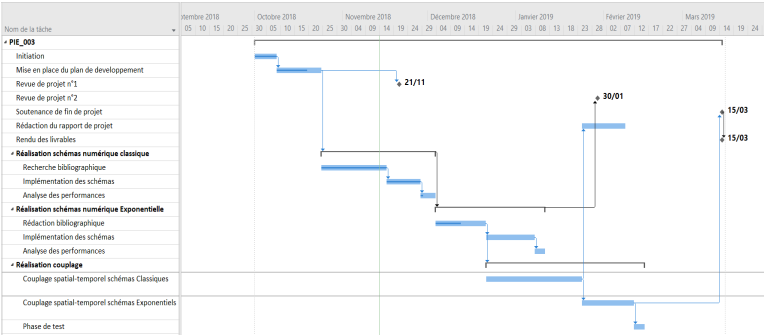
\includegraphics[width=\textwidth]{images/gantt.png}
            \caption{Diagramme de Gantt initial} 
            \label{fig:Gantt_initial}
        \end{figure}

    \subsubsection{Planning de projet}
        \paragraph{}
        Après plusieurs entretiens avec le client, nous avons convenu de plusieurs changements qui ont provoqués des différences majeures dans l'emploi du temps du projet. 

        \paragraph{}
        Nous nous occupons de la partie intégration temporelle, néanmoins cette partie doit être couplée avec les méthodes d'intégration spatiales. Ces méthodes ont été réalisées au préalable par d'autres groupes d'étudiants de Supaero dans les années antérieures. Pour l'équipe couplage, il s'est avéré difficile de reprendre le code informatique tel qu'il nous était fourni pour le coupler avec notre travail sur l'intégration temporelle. Après discussion avec nos clients, nous avons donc réussi à les convaincre de changer la structure du code afin qu'il soit plus flexible et utilisable qu'avant.

        \paragraph{}
        Cette tâche supplémentaire était un risque très important pour notre projet. Car le code informatique étant fonctionnel, nous risquions le dégrader et le rendre inutilisable. Dans un second temps cette tâche n'était pas prévue dans le diagramme de Gantt initial. Il y avait donc un risque de passer trop de temps sur cette opération et compromettre l'ensemble du projet.
        \begin{figure}
            \centering
            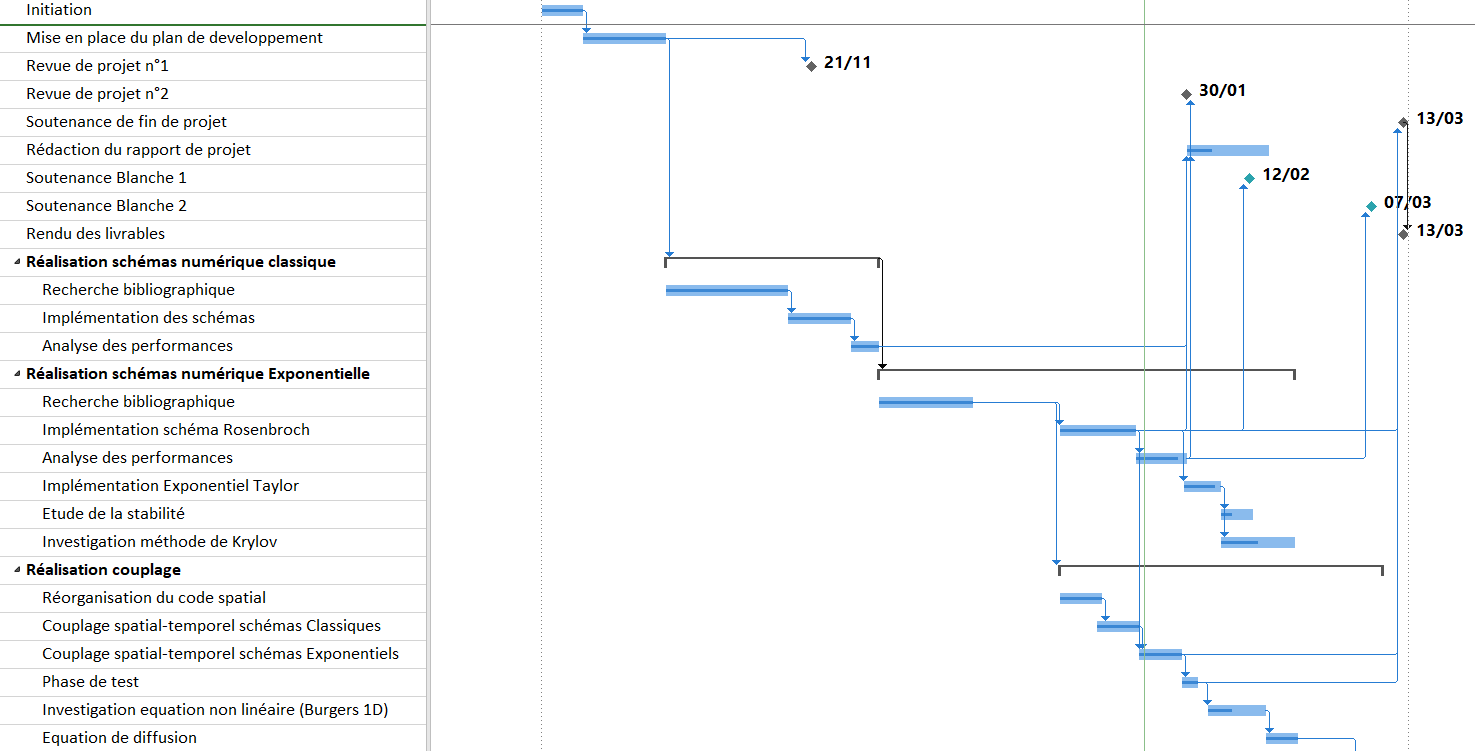
\includegraphics[width=\textwidth]{images/gantt_2.png}
            \caption{Diagramme de Gantt modifié} 
            \label{fig:Gantt modifié}
        \end{figure}

        \paragraph{}
        Finalement, comme nous pouvons le voir sur la figure \ref{fig:Gantt modifié} ce risque s'est transformé en opportunité, car la tâche a été effectuée rapidement et avec succès ce qui a permit à l'équipe couplage de gagner un temps considérable sur la suite du projet.

        \paragraph{}
        En parallèle l'équipe développement a eu des difficultés sur l'implémentation des schémas temporels. Le travail de l'équipe couplage étant conditionné par la réussite de l'équipe développement nous avons fait le choix de déplacer une ressource humaine dans l'équipe implémentation. Nous avons donc globalement pris de l'avance sur les objectifs initiaux fixés du projet. 

        \paragraph{}
        Le diagramme de Gantt est l'outil principal que nous avons utilisé tout au long du projet. Il permet de situer temporellement parlant le travail effectué par rapport aux prévisions, ce qui est très utile quand les demandes du client évoluent au cours du projet.

        \paragraph{}
        Le client a par exemple exigé des soutenances de projet "blanches" mi-février et début mars. Ceci nous a donc imposé de préparer des présentations orales supplémentaires et d'arranger la répartition du travail de façon à avoir de nouveaux  résultats à montrer au client lors de la soutenance. Ces aléas d'emploi du temps ont été très bien gérés par l'équipe grâce au diagramme de Gantt. Ces modifications apparaissent en comparant les figures \ref{fig:Gantt_initial} et \ref{fig:Gantt modifié}.


\subsection{Coût réel du projet}

    \paragraph{}
    Comme nous avons pu le voir, nous avons gagné du temps sur certaines tâches ce qui nous a permis d'aller plus loin que ce que le client demandait initialement. Néanmoins ce surplus de tâches nous a fait dépasser le nombre d'heures alloué à ce projet d'environ 20\%. Ce qui fait un total de 480h pour ce projet. En considérant la rémunération minimale d'un stagiaire qui est de 3,72 euros par heure net, le montant du projet s'élèverait à 1785,6\euro auquel s'ajouterait les charges patronales. Considérons maintenant un salaire de jeune ingénieur à la sortie de l'école ISAE-SUPAERO en se basant sur un revenu annuel de 40 000\euro brut par an. En considérant des charges patronales de l'ordre de 30\%, le montant du projet s'élèverait cette fois-ci à 9984\euro. Il faut souligner le fait que nous avons été plus loin que les objectifs initiaux et que par conséquent le prix du projet s'en fait ressentir dans la globalité.


\subsection{Les livrables du projet}

    \subsubsection{Liste des produits livrables au client}
        \paragraph{}
        Les livrables du projet sont :
        \begin{itemize}
            \item une revue bibliographique avec pour objectif de répondre aux questions : \textit{quelles méthodes est-il conseillé d'utiliser, pourquoi et pour quelles applications ?}
            \item un rapport de projet (le présent document)
            \item un rendu des supports utilisés pour la soutenance finale
            \item le code informatique avec pour critère d'acceptation d'être fait en langage Python et publié sur la plateforme GitHub
        \end{itemize}

    \subsubsection{Liste des livrables demandés par le corps enseignant}
        \paragraph{}
        Dans le cadre du module de gestion de projet de l'ISAE Supaero, nous devons rendre un plan de développement de notre projet. D'autre part nous sommes évalués sur un rapport de projet et une soutenance qui aura lieu mi-mars. Ce sont donc des livrables requis.

        \paragraph{}
        Un dernier livrable requis est une fiche synthèse, format A4, résumant brièvement les enjeux du projet et les résultats obtenus. 


\subsection{Risques et opportunités}

    \paragraph{}
    Les risques liés au projet sont répertoriés dans le tableau présenté en figure \ref{Tab risque}. On peut voir que ce tableau est réalisé en définissant pour chaque risque potentiel une occurrence et une gravité à travers un coefficient. Le produit de ces deux coefficients nous indiquera tout naturellement si l'impact du risque considéré sur le projet est fort ou non. L'utilisation d'un code couleur permet ensuite de repérer visuellement les risques majeurs d'un simple coup d'oeil.

    \paragraph{}
    Une fois ces risques identifiés, il est à notre charge de faire en sorte qu'ils ne se produisent pas. C'est donc ce que nous nous sommes efforcés de faire tout au long du projet. Bien sûr ayant une faible expérience en gestion de projet, il est difficile d'identifier en amont tous les risques qu'un projet peu présenter.

    \paragraph{}
    Il y a d'ailleurs un risque que nous n'avions pas considéré : l'incompatibilité ou la difficulté du couplage de notre travail avec la méthode spatiale. En effet, la méthode spatiale étant fournie par le client, nous avons récupéré un code informatique fonctionnel. Néanmoins ce code était réalisé de manière peu flexible et était de mauvaise qualité (d'un point de vue informatique, et pas algorithmique) ce qui ne permettait pas de coupler les deux travaux de façon simple et agile.

    \paragraph{}
    C'est alors qu'un choix s'offrait à nous : soit prendre le temps de réécrire la partie du code fournie par le client et avoir la garantie d'avoir un résultat, soit avoir des difficultés pour tester les fruits de notre travail de recherche au risque que cela nous prenne beaucoup de temps. Nous avons préféré, avec l'accord du client, reprendre la structure du code fournit afin de pouvoir effectuer un couplage de notre travail de manière propre et efficace.

    \paragraph{}
    Ce qui s'apparentait à un risque s'est transformé en opportunité car finalement, par rapport au diagramme de Gantt initial, nous avions gagné du temps. Cela nous as ensuite permis de faire plus de choses et de réellement pousser notre travail.
    \begin{figure}
        \centering
        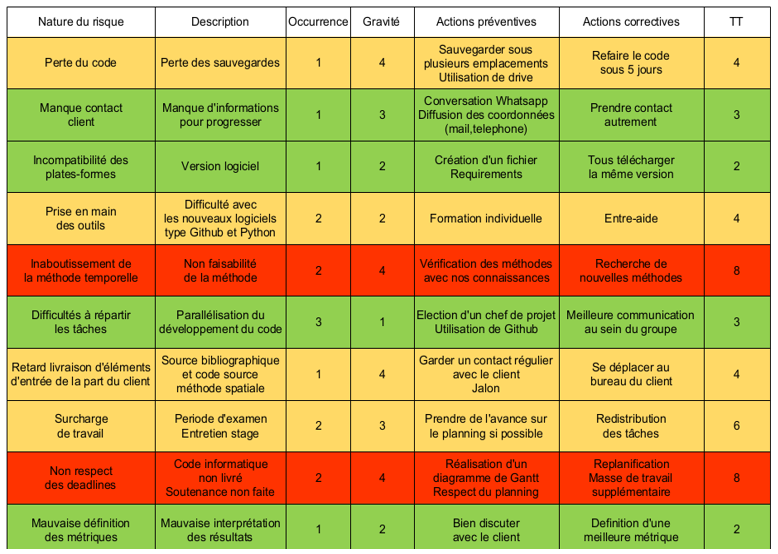
\includegraphics[width=\textwidth]{images/matrice_risque.png}
        \caption{Tableau des risques}
        \label{Tab risque}
    \end{figure}


\subsection{Suivi et Contrôle}

    \subsubsection{Tableau de bord de suivi}
        \paragraph{}
        Nous avons l'opportunité d'utiliser le logiciel MS-Project pour réaliser un suivi du projet. Nous avons réalisé un diagramme de Gantt de référence que nous avons mis à jour au fur et à mesure que le projet évoluait. Cela nous a été très utile car comme nous l'avons vu précédemment nous avons pu réagir vite à des problèmes rencontrés lors du projet.

        \paragraph{}
        Avec l'élaboration du WBS nous avions pu mettre un coût sur chaque tâche à réaliser, et le diagramme de Gantt à mis en évidence qu'en fin de projet, des personnes seraient en surcharge de travail. Nous nous sommes donc efforcés dès le début du projet à ré-agencer les tâches, mais les aléas du projet nous ont aussi aidé à résoudre ce problème.  

        \paragraph{}
        L'utilisation de la plate-forme GitHub, gérant le versionnage des fichiers, possède certaines fonctions aidant aussi à la gestion du projet. On peut rapidement voir quelle personne travaille sur quelle partie du code. Pour le partage de documents, nous avons créé un groupe sur un site de stockage et de partage de documents.

        \paragraph{}
        Ce sont autant de plate-formes qui permettent de garder l'ensemble de l'équipe en contact. Cela a aussi tendance à créer une émulsion et une dynamique de groupe. Néanmoins il faut veiller à ne pas avoir trop d'outils pour ne pas se perdre. Mais dans notre cas chacune des interfaces avait une fonction différente et bien définie

    \subsubsection{Communication}

        \paragraph{}
        De façon à être dynamiques au sein du groupe nous avons mis en place une conversation WhatsApp. L'interface utilisée pour cette application étant le smartphone, cela permet rapidement d'échanger des informations, ou de se donner rendez-vous pour travailler. Notre client est d'ailleurs membre de cette conversation, ce qui lui permet de rester en permanence au courant de l'avancée de notre travail.

        \paragraph{}
        Néanmoins, d'un point de vue plus formel, il nous paraissait très important d'utiliser les mails. C'était de plus le seul moyen de communication avec certaines parties prenantes du projet.

        \paragraph{}
        D'autre part, en moyenne, nous avions décidé de faire des réunions bimensuelles dès le début du projet. Sur l'ensemble du projet il s'agit d'une contrainte que nous nous sommes imposés mais qui fût respectée et nous a permis de rester à l'écoute de notre client concernant ses exigences, qui ont évoluées au cours du temps.


\section{Méthodes numériques}
\subsection{Introduction}
Dans le contexte des projets industriels, la réalisation de campagnes de tests pour dimensionner les systèmes engendre des coûts très importants. Par conséquents des modèles physiques sont de plus en plus utilisés durant les phases de conception des produits dans l'optique de limiter le plus possible les tests en laboratoire et de circonscrire dans la mesure du possible leur utilisation aux seules phases de certifications.\\

Les phénomènes physiques étudiés sont modélisés mathématiquement au moyen d'Equations au Dérivées Partielles (EDP), qui ont pour objet de lier les variations spatiales et temporelles des quantités observées.

A titre d'exemple, les équations de Navier-Stokes conservatives, qui modélisent un écoulement fluide, peuvent s'écrire de la manière suivante:

\begin{equation}
    \frac{\partial W}{\partial t} + \nabla . F(W) -\nabla\left( G(W,\nabla W)\right)=0
    \label{eq:NS}
\end{equation}

où $W$ représente le vecteur d'état (vitesse d'écoulement, énergie...), $F$ donne le flux de ce vecteur d'état et $G$ est un terme de viscosité.\\

En règle général on ne dispose pas de solution analytique des EDP pour des conditions initiales et des conditions de bords quelconques. C'est pour cela que l'on introduit les simulations numériques qui permettent de calculer des solutions approchées de ses équations.\\

Le projet sur lequel nous sommes intervenus se focalise sur le développement d'un code dit de \emph{Computational Fluid Dynamics} (CFD) qui s'intéresse spécifiquement à ces problèmes de modélisation d'écoulement fluide.\\

Lorsqu'on ne prend pas en compte le terme visqueux dans l'équation (\ref{eq:NS}) et qu'on se place en dimension 1D, cette équation se ré-écrit sous la forme d'une équation d'advection:

\begin{equation} 
    \frac{\partial W}{\partial t}+\frac{\partial \mathrm{F}(W)}{\partial x}=0
    \label{eq:advct}
\end{equation}

Cette équation simplifiée du modèle précédent nous a servi de cas test basique tout au long de notre étude car elle présente l'avantage d'être à la fois proche des problématiques de dynamique des fluides de nos clients ainsi que de posséder des solutions analytique ce qui nous a permis d'évaluer la pertinence de nos méthodes numériques.
%idée général des coût de test phy élevés donc simu
%modélisation de la physique par les EDP
%approche numérique si trop complexe pour avoir une sol analytique
\subsubsection{Couplage spatio-temporel}
Il est possible d'isoler dans les équations que nous étudions ici une partie traitant de l'évolution temporelle et une partie se focalisant sur les variations spatiales. Il est notamment possible de reformuler l'équation (\ref{eq:advct}) de la manière suivante:

\begin{equation}
\frac{\partial W}{\partial t} = -\frac{\partial F(W)}{\partial x}
\label{eq:SpTmp}
\end{equation}

la partie temporelle étant contenue dans le membre de gauche et la partie spatiale dans le membre de droite.

En règle générale, les démarches numériques exposées dans la littérature se focalisent en premier lieu sur l'un ou l'autre de ces aspects.

En ce qui concerne le code développé dans le cadre du projet JAGUAR de notre client c'est l'aspect spatial qui a été particulièrement étudié au travers des méthodes de \emph{Spectral Difference}, exposées dans la sous-section suivante. L'objet d'un PIE précédent consistait précisément à implémenter une méthode de discrétisation de l'opérateur différentiel spatial du membre de gauche de l'équation (\ref{eq:SpTmp}).

Une fois cette étape de discrétisation spatiale réalisée, on peut se ramener à l'étude d'une Equation Différentielle Ordinaire (EDO) de la forme:

\begin{equation}
\left\{
    \begin{aligned}
    \dot{u} = f(t,u)&\\
    u(0) = u_0, &\quad u_0\in \mathbb{R}^n
    \end{aligned}
    \right.
    \label{eq:EDO}
\end{equation}

%Comme expliqué précédemment, notre objectif était de trouver une méthode temporelle en adéquation avec la précision des méthodes spatiales développées par le client. Vérifié la validité du couplage spatio-temporel des différentes méthodes considérées ici faisait donc partie des enjeux cruciaux pour satisfaire notre client.\\
C'est la possibilité d'étudier en parallèle à la fois de nouvelles méthodes numériques temporelles ainsi qu'un traitement du couplage spatio-temporel qui a motivé notre choix de nous répartir en deux équipes distincts.

Dans la suite du rapport sont donc exposés en premier lieu les méthodes de différences spectrales, puis rappels sur les méthodes numériques d'intégration des EDO classiques suivi par l'étude des méthode d'intégrations exponentielles plus récentes et enfin les résultats que nous avons obtenu après implémentation.
%description des eq du problème,
%séparation spatio-temp, en général étudié spéparement
%réduction au EDO
\subsubsection{Notions essentielles d'analyse numérique}
Comme mentionné précédemment, l'utilisation de schémas numériques est souvent indispensable aussi bien pour la résolution d'EDP que pour la résolution d'EDO. Avant de passer au parties suivantes, nous rappelons ici quelques notions essentielles d'analyse numérique.\\

On se place ici dans le cas très simple où l'on considère le problème suivant:
\begin{equation}
\left\{
    \begin{aligned}
        \dot{u} = A u, \quad  A \in \mathcal{M}_n(\mathbb{R})\\
        u(0) = u_0, \quad u_0 \in \mathbb{R}^n
    \end{aligned}
\right.
\label{eq:lin}
\end{equation}

Cette équation différentielle ordinaire à pour solution la fonction
$$
u(t) = e^{A t}u_0, \quad t\in \mathbb{R}
$$
et est stable ssi son spectre est inclus dans le demi-plan gauche de l'espace complexe $\mathbb{C}$ (i.e. $\forall \lambda \in \sigma(A), Re (\lambda) \leq 0$). Si les valeurs du spectre sont strictement contenues dans $\mathbb{C}^- = \{z\in \mathbb{C}, Re(z)<0\}$, alors la solution du problème est asymptotiquement stable et converge exponentiellement vite vers $0$.\\

Une façon intuitive de discrétiser le problème selon un pas de temps $\Delta t$ est la suivante:
\begin{equation}
    \frac{u_{n+1}-u_n}{\Delta t} = A u_n 
    \label{eq:Euler}
\end{equation}
Il s'agit du schéma d'Euler.

En posant pour $n\in \mathbb{N}$ $t_n = n \Delta t$, on peut montrer par un développement limité qu'une solution du problème (\ref{eq:lin}) vérifie:
$$
\frac{u(t_{n+1}) -u(t_n)}{\Delta t} = \frac{1}{\Delta t}\left(u(t_n) + \Delta t \dot{u}(t_n) +o(\Delta t) - u(t_n)\right) = Au_n +o(1)
$$
Autrement dit une solution de (\ref{eq:lin}) vérifie le schéma (\ref{eq:Euler}) à un terme résiduel prés qui converge vers 0 lorsque $\Delta t \rightarrow 0$. Réciproquement, on peut montrer qu'une fonction vérifie l'équation (\ref{eq:Euler}) seulement si elle vérifie à un terme résiduel près le système (\ref{eq:lin}). Cela caractérise la notion de \emph{consistance} qui représente intuitivement la capacité du schéma numérique à bien restituer le comportement local des solutions que l'on cherche à simuler lorsque l'on fait tendre le pas de temps $\Delta t$ vers.\\

Cette erreur locale sera inévitablement reproduite à chaque itération de notre schéma numérique et s'accumulera progressivement. On peut cependant attendre du schéma qu'il n'amplifie pas déraisonnablement cet écart. C'est ce qui correspond intuitivement à la notion de \emph{stabilité}.  
%rappel utilité
%cas très simple
%convergence: notions de stabilité et de consistance
%deux grandes approches: explicite vs implicite
\subsection{Méthodes spectrales}

\paragraph{}
Les méthodes spectrales ont été le sujet d'un précédent PIE, sur lequel nous nous basons dans le cadre de notre travail. Dans cette partie nous allons présenter certaines propriétés de la méthode des différence spectrales (méthode SD).

    \subsubsection{Intérêt}
    \paragraph{}
    Les méthodes spectrales se distinguent des autres méthodes car elles permettent de conserver des propriétés physiques des phénomènes étudiés. Notamment en mécanique des fluides une des propriétés importante est la conservation du flux. Cette méthode permet aussi un gain de temps de calcul considérable par rapport au différence finies. Et les performances d'un solveur étant en partie lié à la rapidité de résolution on comprend l'intérêt porté à ces méthodes.
    \paragraph{}
    En terme de précision nous pouvons obtenir des ordres très élevés avec ces méthodes. Car on cherche la solution sous forme d'une combinaison linéaire sur des fonctions de base et que ces fonctions sont définies par cellules. 

    \subsubsection{Formalisme et Définition}
    \paragraph{}
    Comme nous l'avons vu les méthodes spectrales permettent d'assurer la continuité du flux aux interfaces. Elles sont donc particulièrement intéressantes dans les cas des EDP de type conservatives, rencontrés dans les problèmes de nos clients. Par exemple on peut considérer l'équation aux dérivées partielles suivante en 1D :
    $$\frac{\partial W}{\partial t} + \frac{\partial \mathrm{F}\left(W\right)}{\partial x} = 0$$
    On retrouve l'équation \ref{eq:advct}, où $W$ est la grandeur considérée et F le flux qui dépend de $W$.
    \paragraph{}
    Les méthodes spectrales supposent quand dans chaque cellule du domaine de calcul il y ait p + 1 degrés de liberté pour définir la solution ainsi que q + 1 degrés de liberté pour définir le flux. A un instant donné, les grandeurs F et $W$ sont approximées par des fonctions polynomiales $\mathrm{F}_N$ et $W_N$ dans la cellule $N$. Ce sont alors des polynômes de degrés respectifs p et q :
    \begin{equation}
    \begin{split}
        W_N\left(x, t\right) &= \sum_{i = 0}^p w_i\left(t\right)x^i \\
            \mathrm{F}_N\left(x, t\right) &= \sum_{i = 0}^q a_i\left(t\right)x^i
    \end{split}
    \label{eq:sol_flux_as_polynomials}
    \end{equation}
    \paragraph{}
    La résolution du problème dans chaque maille ne se fait pas dans l'espace réel mais dans un espace isoparamétrique, qui est normalisé. Dans notre cas, la cellule isoparamétrique est le segment [-1, 1] et le passage d'un espace à l'autre s'effectue par une homothétie et une translation. 
    \paragraph{}
    Des propriétés importantes de ce formalisme sont établies : 
    \begin{itemize}[label=\textbullet]
           \item Consistance du schéma : l'approximation polynomiale (équation \ref{eq:sol_flux_as_polynomials}) et l'équation du problème (équation \ref{eq:advct}) impliquent une condition sur les degrés des polynômes solution et flux : q~=~p~+~1
           \item Conservation du flux : il faut que le flux se conserve aux interfaces, il vient donc : $\mathrm{F}_{N-1}(1)=\mathrm{F}_{N}(-1)$ et $\mathrm{F}_{N}(1)=\mathrm{F}_{N+1}(-1)$
    \end{itemize}
    \begin{figure}
        \centering
        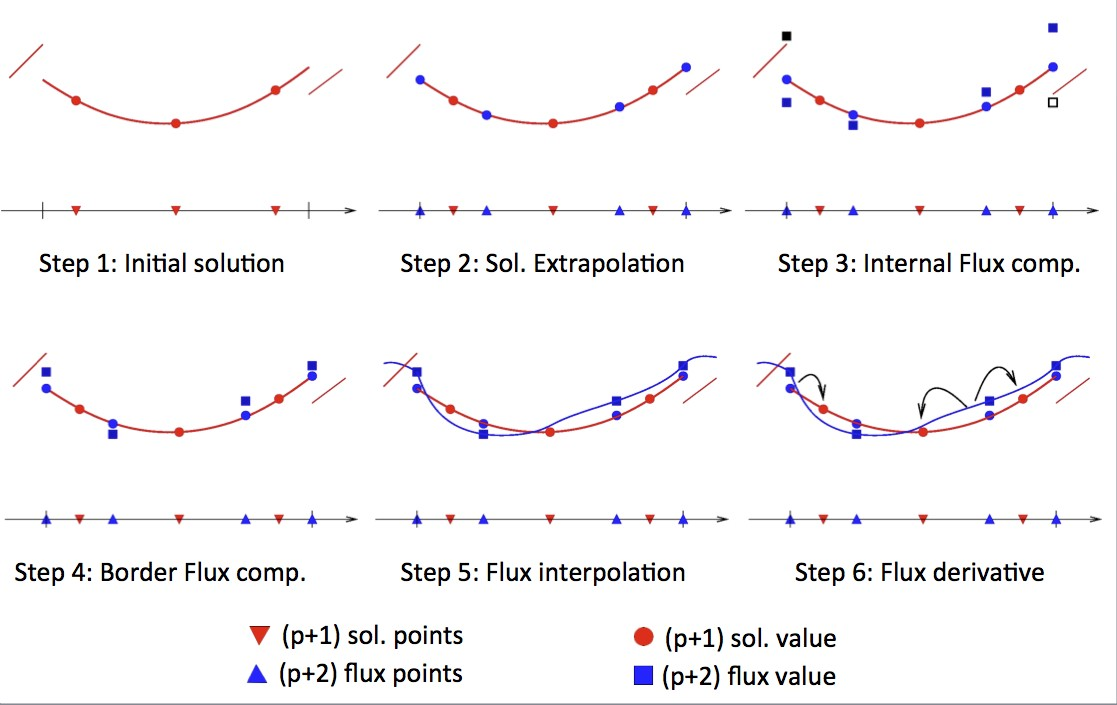
\includegraphics[width=0.8\textwidth]{images/Meth_spectrale.jpg}
          \caption{Schématisation de la méthode} 
    \label{fig:meth_spectrale}
    \end{figure}
    \paragraph{}
    Une brève description de la méthode, illustrée par la figure \ref{fig:meth_spectrale}, permettra de comprendre le fonctionnement.\\
    \textbf{Étape 1 :} Initialisation de la solution dans la cellule avec un polynôme de degré p aux p~+~1 points solution\\
    \textbf{Étape 2 :} Extrapolation de la solution aux p~+~2 points flux, intercalés entre les p~+~1 points solution et positionnés aux extrémités de la cellule, par le polynôme de degré p basé sur la solution\\
    \textbf{Étape 3 :} Calcul du flux aux p~+~2 points flux grâce aux valeurs de la solution interpolée\\
    \textbf{Étape 4 :} Résolution du problème de Riemann pour calculer les flux communs aux interfaces et assurer la continuité du flux sur le domaine\\
    \textbf{Étape 5 :} Interpolation de ce flux continu aux p~+~2 points flux pour obtenir un polynôme de degré p~+~1 le représentant\\
    \textbf{Étape 6 :} Dérivation de ce polynôme de degré p~+~1 pour obtenir un polynôme de degré p représentant la dérivée du flux, et évaluation de ce polynôme en les p~+~1 points solutions\\
    Finalement, on part d'un polynôme représentant $W$ de degré p et on obtient un polynôme représentant la dérivée du flux F lui aussi de degré p.


\subsection{Méthodes temporelles}
\subsubsection{Méthodes classiques}

Dans cette section nous allons présenter les méthodes numériques de résolution temporelles qui sont les plus utilisées à l'heure actuelle. Nous savons que la principale difficulté de ces méthodes est de concilier ordre élevé et stabilité, ce qui permettrai d'augmenter la précision des calculs de logiciel de CFD. \\ 
Pour cela nous allons d'une part étudier une méthode explicite dite de Runge-Kutta (RK) et d'autre part une méthode implicite dite Backward Differentiation Formula (BDF).
La méthode BDF est d'avantage utilisée pour la résolution de phénomènes à évolution rapide qui vont tendre lentement vers une position d'équilibre (équations raides). Tandis que la méthode de Runge-Kutta est plus utilisée pour des problèmes d'advection diffusion. 

\subsubsection{Méthode de Runge-Kutta Explicite (RK)}

Il s'agit d'une méthode d'analyse numérique élaborée par Carl Runge et Martin W. Kutta en 1901.
En tant que méthode explicite, elle détermine la solution à t +  $\Delta$t en fonction de la valeur de la fonction en t. Le problème se formalise de la manière suivante :

\begin{equation}
    y(t + \Delta t) = F(y(t))
\end{equation}

Son caractère explicite donne également qu'elle sera conditionnellement stable. Cela signifie que sous les conditions données par Lax la solution ne convergera que pour des valeurs suffisamment petites de $\Delta$t. De cette manière, le coût de calcul provient du nombre élevé d'itération à cause du petit pas de temps.

Considérons le problème suivant :

\begin{equation}
    y' = f(t, y),    y(t_0) = y_0
\end{equation}

Soit $(tn)_{n \in [0, N]}$ une discrétisation de $[t_0, t_N]$ de pas $\Delta t$. En notant $t_{n,i} = t_n + c_i . \Delta t$, on a pour solutions exactes de y :

\begin{equation}
    y(t_{n,i}) = y(t_n) + \Delta t \int_{0}^{c_i} f(t_n + uh_n, y(t_n + uh_n)) \, \mathrm{d}u
\end{equation}
et
\begin{equation}
    y(t_{n + 1}) = y(t_n) + \Delta t \int_{0}^{1} f(t_n + uh_n, y(t_n + uh_n)) \, \mathrm{d}u
\end{equation}

On peut évaluer numériquement ces équations par une méthode de quadrature en introduisant s "étages". Ainsi, la méthode de Runge-Kutta est en quelque sorte une méthode à "sous-pas" multiples. De cette manière et en posant les coefficients $a_{i, k}$ et $b_i$,  on obtient la méthode de Runge-Kutta d'ordre s:

\begin{equation}
    y_{n+1} = y_n + \Delta t \sum_{i=1}^{s} b_ik_i
\end{equation}
avec,\\
    $k_i = f(t_n + c_i\Delta t, y_n + \Delta t \sum_{k=1}^{i-1} a_{i,k}k_k)$

Les coefficients de la méthode sont donnés par le tableau de Butcher. Nous remarquerons que la méthode de Runge-Kutta à l'ordre 1 (RK1) est le schéma d'Euler explicite.

La méthode usuelle de Runge-Kutta explicite est la méthode d'ordre 4 (RK4) qui est donnée par l'équation suivante:

\begin{equation}
    y_{n+1} = y_n + \frac{\Delta t}{6}(k_1 + 2k_2 + 2k_3 + k_4)
\end{equation}
où,\\
$k_1 = f(t_n, y_n)$\\
$k_2 = f(t_n + \frac{\Delta t}{2}, y_n + \frac{\Delta t}{2}k_1)$\\
$k_3 = f(t_n + \frac{\Delta t}{2}, y_n + \frac{\Delta t}{2}k_2)$\\
$k_4 = f(t_n + \Delta t, y_n + \Delta tk_3)$

Cette méthode est d'ordre 4, ce qui signifie que l'erreur totale accumulée est de l'ordre de $\Delta t^4$.

\begin{figure}[h]
    \centering
    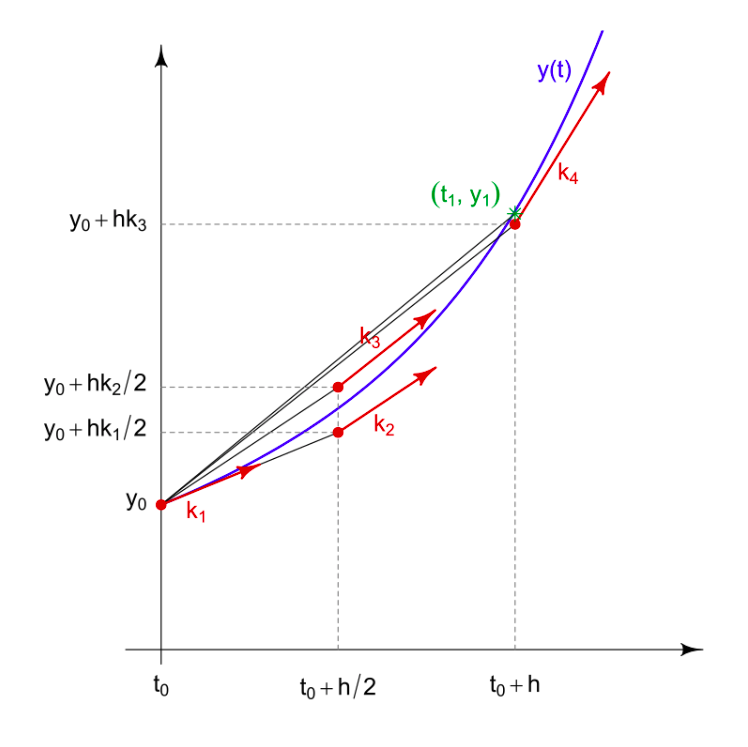
\includegraphics[width=0.5\textwidth]{images/RK_pentes.png}
    \caption{\textit{Slopes used by the classical Runge-Kutta method}, HilberTraum}
\label{fig:pentes_rk}
\end{figure}

La figure \ref{fig:pentes_rk} nous permet de réaliser que $y_{n+1}$ est calculé comme étant la somme $y_n$ et du produit entre $\Delta t$ et la pente approchée par la moyenne pondérée des pentes $k_i$. De cette manière :
\begin{itemize}
    \item $k_1$ est la pente au début de l'intervalle
    \item $k_2$ est la pente au milieu de l'intervalle en utilisant $k_1$ pour calculer $y(t_n + \frac{\Delta t}{2}$)
    \item $k_3$ est la pente au milieu de l'intervalle en utilisant $k_2$ pour calculer $y(t_n + \frac{\Delta t}{2}$)
    \item $k_4$ est la pente à la fin de l'intervalle
\end{itemize}

Le comportement des méthodes numériques sur les équations raides peut être analysé en appliquant ces méthodes à l'équation de test $y' = Ay$ sous réserve de la condition initiale y(0) = 1 avec $A \in \mathbb{C}$. La solution de cette équation est $y (t) = e^{At}$. Cette solution se rapproche de zéro lorsque t tend vers l'infini si $\mathrm{Re}(A)<0$. Si la méthode numérique présente également ce comportement, alors la méthode est dite A-stable.

\begin{figure}[h!]
    \centering
    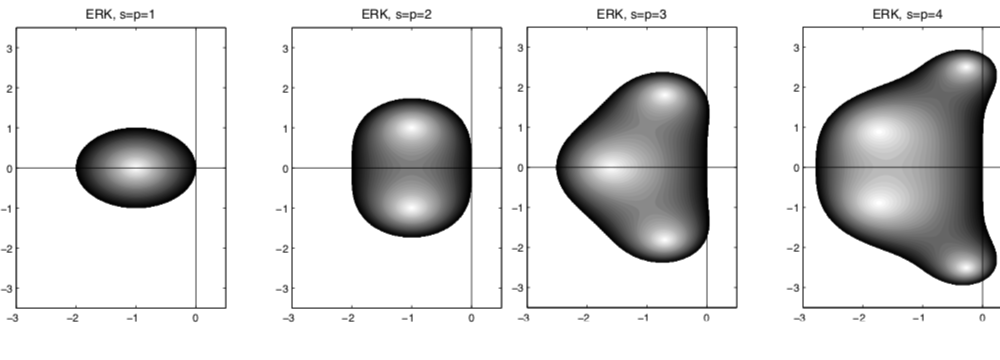
\includegraphics[width=\textwidth]{images/astab_rk.png}
    \caption{\textit{Stability of Runge-Kutta Methods}, Utrecht University}
\label{fig:astab_rk}
\end{figure}

La partie grisée de la figure \ref{fig:astab_rk} indique les valeurs de A pour lesquelles la solution numérique de y tend vers 0 respectivement sous RK1, RK2, RK3 et RK4. On remarque donc que la méthode de Runge-Kutta est conditionnellement A-Stable quelque soit son ordre. Pour cette raison, nous allons introduire une autre méthode d'analyse numérique usuelle afin d'obtenir une stabilité inconditionnelle et pouvoir traiter les cas raides.

\subsubsection{Méthode de Backward Differentiation Formula (BDF)}

Il s'agit d'une méthode d'analyse numérique élaborée par Charles F. Curtiss et Joseph O. Hirschfelder en 1952.
En tant que méthode implicite, elle détermine la solution à t +  $\Delta$t en résolvant une équation prenant en compte la valeur de la fonction en t et en t +  $\Delta$t. Le problème se formalise de la manière suivante : 

\begin{equation}
    G(y(t), y(t+\Delta t)) = 0
\end{equation}

Son caractère implicite donne également qu'elle sera inconditionnellement stable, en tout cas pour les méthodes d'ordre inférieur ou égal à 2. De cette manière, le coût de calcul provient de l'évaluation numérique de la racine de G, par une méthode de Newton par exemple.

Considérons le problème suivant :

\begin{equation}
    y' = f(t, y),    y(t_0) = y_0
\end{equation}

La méthode BDF est quand à elle une méthode à pas multiples. En posant les coefficients $a_k$ et $\beta$,  on obtient la méthode de BDF d'ordre s:

\begin{equation}
    \sum_{i=1}^{s} a_k y_{n+k} = \Delta t \beta f(t_{n+s}, y_{n+s})
\end{equation}

Les coefficients de la méthode sont donnés par le polynôme d'interpolation de Langrange. Nous remarquerons que la méthode BDF à l'ordre 1 (BDF1) est le schéma d'Euler implicite.

La méthode usuelle BDF est la méthode d'ordre 4 (BDF4) qui est donnée par l'équation suivante:

\begin{equation}
    y_{n+4} - \frac{48}{25}y_{n+3}+\frac{36}{25}y_{n+2}+\frac{16}{25}y_{n+1}+\frac{3}{25}y_n = \frac{12}{25}\Delta tf(t_{n+4}, y_{n+4})
\end{equation}

\begin{figure}[h!]
    \centering
    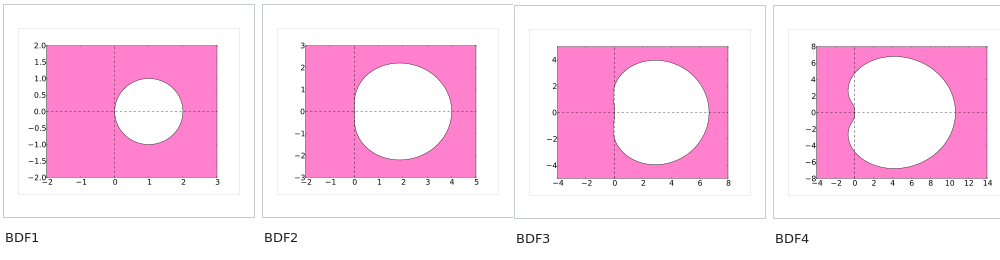
\includegraphics[width=\textwidth]{images/astab_bdf.png}
    \caption{\textit{An Introduction to Numerical Analysis}, Cambridge University Press}
\label{fig:astab_bdf}
\end{figure}

La partie rose de la figure \ref{fig:astab_bdf} indique les valeurs de A pour lesquelles la solution numérique de y tend vers 0 respectivement sous BDF1, BDF2, BDF3 et BDF4. On remarque donc que la méthode BDF est inconditionnellement A-Stable pour un ordre inférieur ou égal à 2 et conditionnellement stable sinon. Malgré cela, la méthode BDF reste plus stable que la méthode RK quelque soit son ordre.
\section{Méthodes exponentielles}
%Tout l'objet de ce projet repose sur ces nouvelles méthodes. La théorie est développée à travers des articles scientifiques très récents. Ce qui montre que c'est un sujet actuelle de recherche, et qu'il y a des possibilités d'amélioration avec ces méthodes. Nous allons vous décrire brièvement le fonctionnement de ces méthodes, puis nous vous montrerons les résultats que nous avons obtenus. 

%mini intro: choisie pour savoir si elle sont prometteuses, rappeler les inconvénients précedent, explicite mais plus grand pas de temps

\paragraph{}
Comme nous l'avons vu dans la partie précédente le défaut principal des méthodes RK et BDF est qu'elles requièrent un temps de calcul important. Soit pour les premières parce qu'elles ne sont pas stable, ce qui implique de devoir prendre un petit pas de temps et réduit fortement le gain obtenu grâce à leur relative simplicité Soit pour les secondes parce que leur stabilité s'obtient au prix de la résolution de systèmes d'équations implicites complexes.

\paragraph{}
Par conséquent tout l'enjeu pour notre client était de trouver des méthodes numériques permettant de concilier un domaine de stabilité suffisant pour pouvoir utiliser un pas de temps conséquent avec la possibilité de conserver des calculs suffisamment simples pour ne pas perdre le gain temporel induit.
A cet égard, les méthodes exponentielles développées récemment et encore peu utilisées dans le cadre des $CFD$ sont particulièrement prometteuses et nous nous sommes orientés vers l'étude de celles-ci sur les conseils de nos tuteurs.

\paragraph{}
Les parties suivantes visent à en exposer les principes fondamentaux ainsi que des possibilités d'implémentation.

\subsection{Re-formulation du problème de base}
On reprend ici le problème général d'équation différentielle ordinaire (\ref{eq:EDO}):
$$
\left\{
    \begin{aligned}
        \dot{u} = f(t,u),&\\
        u(0) = u_0,& \quad u_0 \in \mathbb{R}^n
    \end{aligned}
\right.
$$
L'idée fondamentale des méthodes exponentielles est de séparer le terme de droite, qui représente en général un opérateur différentiel spatial discret ou continu, en une partie linéaire et une partie non-linéaire:
\begin{equation}
    f(t,u) = Au + g(t,u)
\end{equation}
où $A\in \mathcal{M}_n(\mathbb{C}$ et $g$ est une fonction non-linaire (elle peut tout de même être identiquement nulle). Cette décomposition est a priori arbitraire. Elle peut venir naturellement d'un problème physique dont on isole les termes linéaire aussi bien qu'être obtenue en linéarisant l'opérateur $f$. Dans une sous-section future nous détailleront une manière de choisir cette décomposition.

L'intérêt d'avoir décomposé ainsi le membre de droite est que cela permet de mieux prendre en compte la partie linéaire lors du processus d'intégration. En effet on obtient désormais en intégrant le problème (\ref{eq:EDO}) à l'aide la formule de Duhamel:
\begin{equation} 
    u(t)=e^{A(t-t_{0})} u_{0}+\int_{t_{0}}^{t} e^{A(t-s)} g(u(s), s) \text{d} s
\end{equation}
Pour passer de l'étape $t_n$ à l'étape $t_{n+1} = t_n +\tau$ on a alors la formule d'itération (dans le cas de notre discrétisation temporelle $\tau = \Delta t$):

\begin{equation} 
    u\left(t_{n}+\tau \right)=e^{-\tau A} u\left(t_{n}\right)+\int_{0}^{\tau} e^{-(\tau-\sigma) A} g\left(u\left(t_{n}+\sigma\right),t_n+\sigma\right) d \sigma
    \label{eq:itExp}
\end{equation}

Le terme exponentiel $e^{-\tau A} u\left(t_{n}\right)$ permet d'intégrer exactement la partie linéaire. A titre de comparaison, la formule d'intégration qui sert de base au méthodes classiques de Runge-Kutta est la suivante:
$$
u(t_{n+1}) = u(t_n) + \int_{0}^{\tau} f\left(u\left(t_{n}+\sigma\right),t_n+\sigma\right) d \sigma
$$
Dans ce cas l'ensemble de l'information contenue dans le terme de droite était soumise aux imprécisions dues à la méthode de quadrature approchée utilisée pour calculer le terme intégral, alors qu'avec la méthode exponentielle la partie linéaire qui a été isolée est calculée exactement (à la précision d'un calcul d'exponentielle de matrice).

Tout l'enjeu à partir d'ici réside dans le calcul dans le terme d'intégral qui demeure dans la formule (\ref{eq:itExp}) :
$$
\int_{0}^{\tau} e^{-(\tau-\sigma) A} g\left(u\left(t_{n}+\sigma\right),t_n+\sigma\right) d \sigma
$$

\subsection{Calcul de quadrature}
Dans cette sous section nous allons voir deux méthodes pour calculer le terme intégral.
\subsubsection{Méthode Runge-Kutta}
Une idée naturelle pour effectuer ce calcul de quadrature est d'utiliser une méthode inspirée de la démarche de Runge-Kutta puisque celle-ci consiste essentiellement en un calcul d'intégral approché.

La méthode que nous allons décrire ici est entièrement développée dans l'article de Hochbruck \cite{ExpIntegrators}.

On commence par poser dans un premier temps $0 \leq c_1 \leq ... \leq c_s \leq 1$
et on suppose que l'on dispose de valeurs approximées de notre solution en différents points :
\begin{equation}
    U_{n,i} \approx u(t_n + c_i \tau)
\end{equation}

On peut alors définir une approximation de la fonction $u$ à l'instant $t_{n+1}$ de manière analogue à ce qui a été fait dans le cadre de RK:

\begin{equation} 
    \begin{aligned} u_{n+1} &=\mathrm{e}^{-\tau A} u_{n}+\tau \sum_{i=1}^{s} b_{i}(-\tau A) G_{n,i} \\
    G_{n,i} &=g\left(U_{n,i}\right) \\
    U_{n,i} &=\mathrm{e}^{-c_{t} \tau A} u_{n}+\tau \sum_{j=1}^{s} a_{i,j}(-\tau A) G_{n,j} \end{aligned}
\end{equation}
Ici seule l'intégrale en $g$ fait l'objet d'une approximation, le l'exponentielle de matrice est bien calculée exactement. Le lecteur averti pourra également remarquer que dans le cas où l'on prend $A=0$ et $g=f$, on retrouve alors précisément les formules de RK évoquées plus haut (avec $b_i(0)$ et $a_{i,j}(0)$ comme coefficient).

Il faut maintenant trouver des relations sur les coefficients de ces formules. Pour cela une démarche naturelle consiste à les choisir de sorte que la formule de quadrature soit exacte lorsque la fonction $g$ est identiquement constante. Dans ce cas on a :
\begin{equation} 
    u\left(t_{n}+\theta \tau\right)=e^{-\theta \tau A} u\left(t_{n}\right)+\theta \tau \varphi_{1}(-\theta \tau A) g
\end{equation}
où
\begin{equation} 
    \varphi_{1}(z)=\int_{0}^{1} \mathrm{e}^{(1-\sigma) z} d \sigma=\frac{\mathrm{e}^{z}-1}{z}
\end{equation}
En utilisant cette formule pour $\theta = c_1,...,c_s$ et pour $\theta = 1$ alors les conditions
$$
u_n = u(t_n),\quad U_{n,i} = u(t_n+c_i \tau), \quad n\in \mathbb{N}, i\in\{1,...,s\}
$$
sont vérifiées si les hypothèses simplificatrices suivantes sont faites:
\begin{equation} 
    \begin{array}{l}{\sum_{i=1}^{s} b_{i}(z)=\varphi_{1}(z)} \\ {\sum_{j=1}^{s} a_{i j}(z)=c_{i} \varphi_{1}\left(c_{i} z\right), \quad i=1, \ldots, s}\end{array}
\end{equation}
Cependant, cela laisse un très large choix d'implémentations possibles.
\subsubsection{Méthode Taylor exponentielle}

Une autre manière de calculer le terme intégral est d'utiliser un développement de Taylor de la fonction $d$. Cette méthode est développée dans l'article \cite{Taylor}.

L'approximation faite consiste donc à écrire:
\begin{equation} 
    g(\tau, u(\tau)) \approx \sum_{k=0}^{p-1} \frac{\left(\tau-t_{0}\right)^{k}}{k !} \frac{\mathrm{d}^{k}}{\mathrm{d} t^{k}} g\left.(t, u(t))\right|_{t=t_{0}}
\end{equation}

En utilisant des coefficients tels que

\begin{equation} 
    w_{k} \approx \frac{\mathrm{d}^{k-1}}{\mathrm{d} t^{k-1}} g\left.(t, u(t))\right|_{t=t_{0}}
\end{equation}
(l'obtention de ces coefficients est détaillée dans \cite{Taylor}) on peut alors intégrer exactement l'approximation polynomiale de $g$
\begin{equation} 
    u_{n+1}=\mathrm{e}^{\tau A} u_{n}+\sum_{k=1}^{p} \tau^{k} \varphi_{k}(\tau A) w_{k} = u_{0}+\tau \varphi_{1}(\tau A) f\left(t_{0}, u_{0}\right)+\sum_{k=2}^{p} \tau^{k} \varphi_{k}(\tau A) w_{k}
\end{equation}

où

\begin{equation} 
    \varphi_{k}(z)=\int_{0}^{1} \mathrm{e}^{(1-\theta) z} \frac{\theta^{k-1}}{(k-1) !} \mathrm{d} \theta \quad k \geq 1
\end{equation}

\subsubsection{Lien à l'ordre 1}
On peut relever que à l'odre 1, c'est à dire $s=1$ pour RK ou $k=1$ pour Taylor, c'est deux méthodes sont identiques:
\begin{equation} 
    \begin{aligned} u_{n+1} &=\mathrm{e}^{-\tau A} u_{n}+\tau \varphi_{1}(-\tau A) g\left(t_{n}, u_{n}\right) \\ &=\left(I-\tau A \varphi_{1}(-\tau A)\right) u_{n}+\tau \varphi_{1}(-\tau A) g\left(t_{n}, u_{n}\right) \\ &=u_{n}+\tau \varphi_{1}(-\tau A) F\left(t_{n}, u_{n}\right) \end{aligned}
\end{equation}
Cette méthode est appelée \emph{Euler exponentielle} du fait de sa grande similitude avec la méthode d'Euler explicite:
$$
u_{n+1} = u_n + \tau f(t_n,u_n)
$$
On voit ici que la nouvelle méthode applique un pas de temps "corrigé" à chaque itération.
\paragraph{}
Compte tenu des contrainte de temps et des dimensions préconisées pour ce rapport, il n'est pas possible de restituer les preuves de stabilité et de convergence de ces deux méthodes. Cependant, c'est preuves sont entièrement détaillées dans \cite{ExpIntegrators} et \cite{Taylor}.
%ne pas oublier de préciser un truc sur les preuves de convergence qui sont trop longue pour être évoquées dans le rapport

\subsection{Choix de la décomposition du terme non-linéaire}
Comme expliqué précédemment, le choix de la décomposition 
$$
f(t,u) = Au+g(t,u)
$$
est a priori totalement arbitraire. Cependant, il existe plusieurs manières d'extraire un terme linéaire de $f$ de façon astucieuse.
%rappel arbitraire, problem phy, linéarisation des éq d'Euler
\subsubsection{Approche exponentielle standard}
La manière la plus simple de choisir A est de prendre le linéarisé (ou Jacobienne) de l'opérateur $f$ par rapport à $u$. Comme son nom l'indique, celui-ci caractérise particulièrement bien l'aspect linéaire de $f$:
\begin{equation} 
    F(u(t))=-A u(t)+g(u(t)), \quad A \approx-\frac{\partial F}{\partial u}\left(u_{0}\right)
\end{equation}
Dans l'approche standard, ce terme est calculer une seule fois lors de la première itération. Cela permet de limiter la quantité de caculs effectuées tout au long du procédé. Cependant, plus on avant dans le temps, moins cette linéarisation est valable a priori.
\subsubsection{Approche exponentielle Rosenbrock}
Une autre possibilité consiste à re-linéariser le problème à chaque étape. Il s'agit de l'approche de Rosenbrock:

\begin{equation} 
    \begin{aligned} F(u(t)) &=-A_{n} u(t)+g_{n}(u(t)) \\ A_{n} &=-\frac{\partial F}{\partial u}\left(u_{n}\right) \end{aligned} \quad n=0,1, \ldots
\end{equation}

On s'attend à ce que cette méthode donne de meilleurs résultats puisqu'elle prend en compte à chaque étape une "bonne" linéarisation du problème et parce que la partie linéarisée est intégrée exactement par les méthodes exponentielles. Cependant, cette méthode nécessite de recalculer la Jacobienne de $f$ à chaque itération, ce qui induit un coût supplémentaire en termes de calculs.

\subsection{Calcul des termes exponentiels}
%lourdeur des calculs, multiplicité des phi
\subsubsection{Matrice augmentée}

\paragraph{}
Comme il a déjà été expliqué plus, par construction, la méthode de Taylor exponentielle requiert d'un certain nombre de dérivées de la partie non-linéaire du terme RHS (de l'anglais \textit{Right Hand Side}). De l'application de la formule de Duhammel sur ce problème il découle que le calcul de la solution se réduit à l'exponentielle d'une matrice Jacobienne augmentée qui contient ces dérivées. Ceci est démontré sur les articles de Koskela et Ostermann \cite{Taylor} et Al-Mohy et Higham \cite{ExpIntegrators}.

Ainsi, un problème qui correspond à :
\begin{equation}
    A \in \mathbb{R}^{n \times n}, \quad W=\left[w_{p}, w_{p-1}, \ldots, w_{1}\right] \in \mathbb{R}^{n \times d}
\end{equation}

Peut être finalement résolu sans besoin de calculer les fonctions $\varphi$ à l'aide de cette matrice augmentée :

\begin{equation} 
    \begin{array}{l}{\widetilde{A}=\left[ \begin{array}{cc}{A} & {W} \\ {0} & {J}\end{array}\right] \in \mathbb{R}^{(n+d) \times(n+d)}, \quad J=\left[ \begin{array}{cc}{0} & {I_{d-1}} \\ {0} & {0}\end{array}\right], \quad v_{0}=\left[ \begin{array}{c}{u_{0}} \\ {e_{d}}\end{array}\right] \in \mathbb{R}^{n+d}}\end{array}
\end{equation}

Et de la formule :

\begin{equation} 
    u_{n+1}=\left[I_{d} 0\right] \mathrm{e}^{\Delta t \widetilde{A}} v_{n}
\end{equation} 

\subsubsection{Méthodes de Krylov}

\paragraph{}
En ce qui suit on présente une petite introduction aux méthodes de Krylov basée sur les articles de Schulze, Schmid et Sesterhenn \cite{Krylov:1} et Saad \cite{Krylov:2}, auxquels le lecteur peut s'adresser pour plus de renseignements.

\paragraph{}
Ces méthodes cherchent à accélérer les calculs des exponentielles de matrices à réaliser pendant l'exécution des méthodes étudiées. On peut partir, alors, de la définition de l'exponentielle d'une matrice :%Pour comprendre l'idée principale des ces méthodes...

\begin{equation} 
    e^{A}=\sum_{k=0}^{\infty} \frac{A^{k}}{k !}
\end{equation}

\paragraph{}
Néanmoins, dans les méthodes exponentielles nous n'avons besoin que de calculer le produit : 

\begin{equation} 
    e^{A}v=\sum_{k=0}^{\infty} \frac{A^{k}}{k !}v
    \label{expxvect}
\end{equation}

\paragraph{}
La forme de \ref{expxvect} nous suggère directement une façon d'approximer sa valeur numériquement : tout simplement, on peut tronquer la série. Le résultat sera alors issu de la combinaison linéaire des éléments de la base d'un espace de Krylov.

\paragraph{}
On définit par l'espace de Krylov de d'ordre $m$ associé à la matrice carrée inversible $A \in \mathbb{R}^{n \times n}$ et $v \in \mathbb{C}^{n}$ par :

\begin{equation} 
    \mathcal{K}_{m}(A, v)=s p a n \left\{v, A v, \ldots, A^{m-1} v\right\}
    \label{KrylovSpace}
\end{equation}

\paragraph{}
L'intérêt de cette méthode dépend entièrement de notre capacité à faire diminuer la taille de cet espace de façon à avoir $m<<n$. Cependant, nous pouvons voir aisément (en appliquant, par exemple, la méthode de la puissance itérée sur la matrice $A$) que la base montrée en \ref{KrylovSpace} n'est pas orthogonale, ni bien conditionnée. 

\paragraph{}
Pour en trouver une base orthogonale et bien conditionnée on fait appel à la décomposition d'Arnoldi.

\vspace{0.3cm}

\fbox{
\begin{minipage}{14 cm}
\textbf{Décomposition d'Arnoldi :} 
\hrule
\hspace{0.2 cm}

$\beta \leftarrow \|\mathbf{v}\|_{2}$ 

$\mathbf{v}_{1} \leftarrow \mathbf{v} / \beta$ 

Répéter pour $j$ de $1$ à $m$ 

\quad \quad $p \leftarrow Av_j$ 

\quad \quad Répéter pour $i$ de $1$ à $j$ 

\quad \quad \quad \quad $h_{i, j} \leftarrow \mathbf{v}_{i}^{\mathrm{T}} \mathbf{p}$ 

\quad \quad \quad \quad $\mathbf{p} \leftarrow \mathbf{p}-h_{i, j} \mathbf{v}_{i}$ 

\quad \quad $h_{j+1, j} \leftarrow \|\mathbf{p}\|_{2}$

\quad \quad $\mathbf{v}_{j+1} \leftarrow \mathbf{p} / h_{j+1, j}$

\end{minipage}
}

\vspace{0.3cm}

\paragraph{}
Outre une base orthonormale du sous-espace de Krylov, l'algorithme d'Arnoldi fournit une matrice supérieure de Hessenberg, $\mathcal{H}_{m}$, de taille $m$, qui constitue (à une petite erreur près) une projection de la matrice $A$ sur cette base. Ainsi : 

\begin{equation} 
    \mathbf{H}_{m} \approx \mathbf{V}_{m}^{\mathrm{T}} \mathbf{A} \mathbf{V}_{m}
\end{equation}

\paragraph{}
Et on peut calculer la projection de $e^{tA} v$ sur $\mathcal{K}_{m}$ grâce à :

\begin{equation} 
    e^{tA} v \approx \beta \mathbf{V}_{m+1} \mathrm{e}^{t \mathbf{H}_{m+1}} \mathbf{e}_{1}
\end{equation}

\paragraph{}
Dont la démonstration peut être trouvée sur Schulze et al. \cite{Krylov:1}.

\paragraph{}
Ce résultat peut être encore amélioré avec un effort computationnel négligeable puisque la décomposition d'Arnoldi nous fournit avec le vecteur $m+1$ de la base. Encore une fois, cette amélioration (implémentée dans le code livré) peut être trouvée sur l'article de Schulze et al. \cite{Krylov:1}, mais elle est expliquée de façon plus étendue sur Saad \cite{Krylov:2}.

\paragraph{}
Étant celui-ci un des derniers points abordés dans le cadre de ce projet, les analyses concernant les avantages et problèmes de la méthode de Krylov ne sont pas totalement complètes, et constituent ainsi l'un des axes d'amélioration les plus prometteurs pour des futures études.

\paragraph{}
Nous allons tout de même essayer de montrer dans la suite les principales observations que nous avons pu faire. Dans cette optique, on s'appuie sur un exemple (figure \ref{fig:BurgersKrylov}) pour lequel on évalue l'erreur provoquée par l'utilisation de ces méthodes (figure \ref{fig:Krylov}) et le gain en temps obtenu (tableau \ref{tab:Krylov}) selon la taille du sous-espace de Krylov choisie. La méthode de référence est l'algorithme \textit{Scaling and Squaring} proposé par Al-Mohy et Higham \cite{scipy}, dont la précision est trés élevée, et qui constitue la méthode par défaut du module Scipy de Python pour le calcul des exponentielles de matrices. 

\begin{figure}[h!]
        \centering
        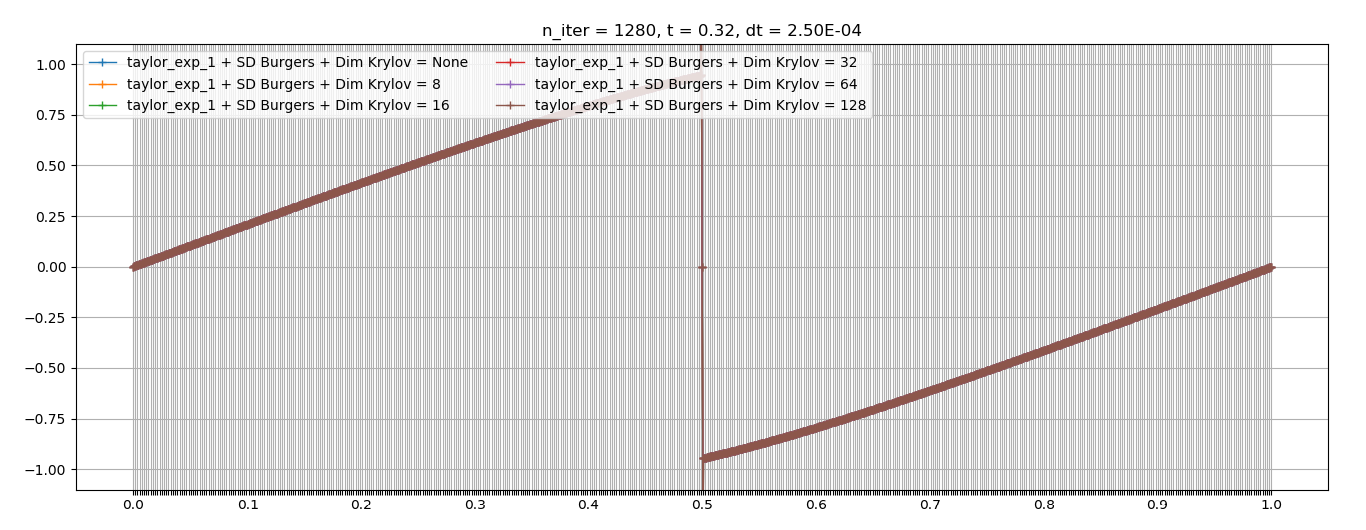
\includegraphics[width=\textwidth]{images/KrylovBurgers.png}
        \caption{Apparition d'une discontinuité dans la solution de l'équation de Burgers avec une condition initiale sinusoïdale, avec $\Delta t = 2.5e-4$, différences spectrales d'ordre 2 sur 511 cellules, exponentielle standard Taylor à l'ordre 1}
        \label{fig:BurgersKrylov}
\end{figure}

\begin{figure}[h!]
        \centering
        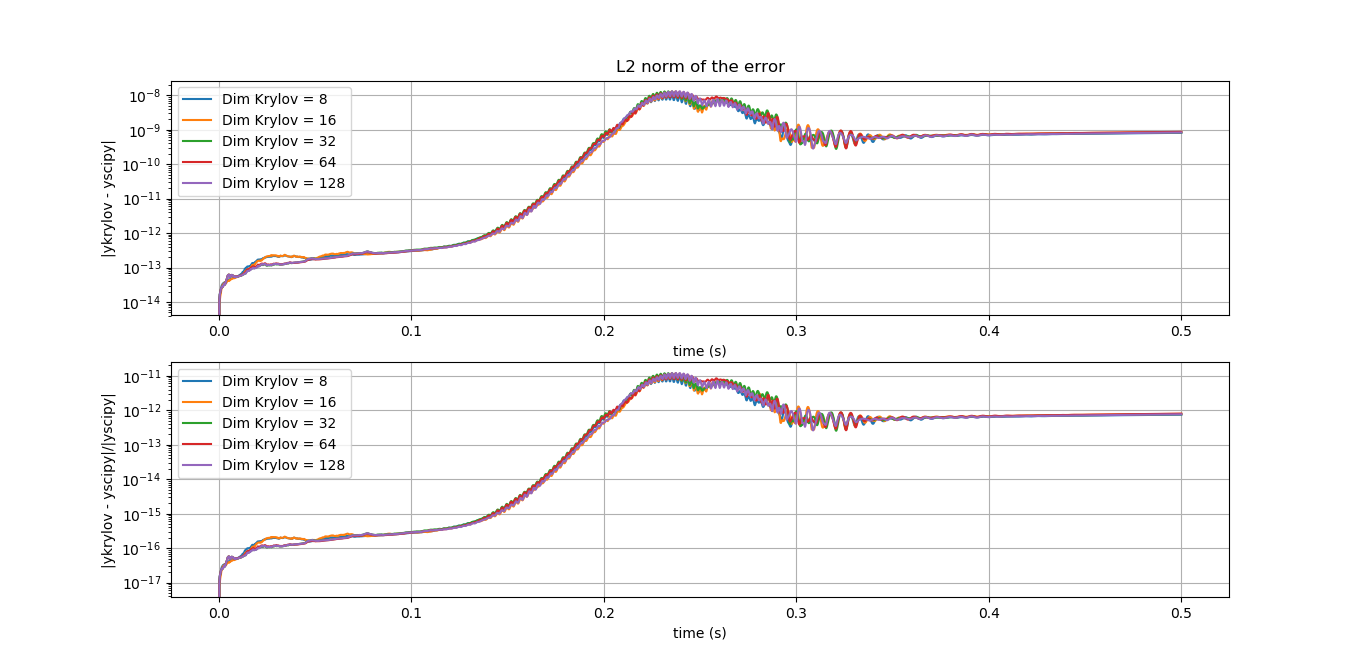
\includegraphics[width=\textwidth]{images/ErreurKrylov.png}
        \caption{Erreur absolue et relative associée à la méthode de Krylov sur l'exemple de la figure \ref{fig:BurgersKrylov}}
        \label{fig:Krylov}
\end{figure}

\begin{table}[h!]
\centering
\begin{tabular}{c|c|c|c|c|c|c|}
\cline{2-7}                            & \multicolumn{1}{c|}{\cellcolor[HTML]{C0C0C0}Scipy} & \multicolumn{1}{c|}{\cellcolor[HTML]{C0C0C0}m = 128} & \multicolumn{1}{c|}{\cellcolor[HTML]{C0C0C0}m = 64} & \multicolumn{1}{c|}{\cellcolor[HTML]{C0C0C0}m = 32} & \multicolumn{1}{c|}{\cellcolor[HTML]{C0C0C0}m = 16} & \multicolumn{1}{c|}{\cellcolor[HTML]{C0C0C0}m = 8} \\ \hline
\multicolumn{1}{|l|}{\cellcolor[HTML]{EFEFEF}temps (s)} & 2726.51 & 90.72 & 109.37 & 145.05 & 225.38 & 458.13 \\ \hline
\end{tabular}
\caption{Temps de calcul associés à l'exemple de la figure \ref{fig:BurgersKrylov}}
\label{tab:Krylov}
\end{table}

\paragraph{}
La première et, probablement, principale remarque est issue du tableau \ref{tab:Krylov} : l'applicabilité des méthodes exponentielles est indissociablement liée à l'utilisation des méthodes de Krylov. Même en 1D et avec une dimension assez réduite, si on cherche à résoudre le problème uniquement à l'aide de la méthode utilisée par Scipy, on obtient des temps de calcul trop élevés pour un code dont un des objectifs est l'application industrielle.

\paragraph{}
On se rend compte aussi que dans ce cas précis les erreurs obtenues, aussi bien celles absolues que celles relatives, restent très faibles au cours du temps. Plusieurs cas test exhibent des comportements très variés qui échappent encore à notre compréhension et pour lesquels nous n'avons pas encore pu trouver d'explication satisfaisante.

\paragraph{}
Il convient d'attirer l'attention sur le fait que, bien que cela ne soit pas clairement visible sur le graphe à cause de la superposition des courbes, l'algorithme utilisée par Scipy n'est pas exempt d'erreurs. Celles-ci semblent se concentrer sur la zone où se situe la discontinuité. Toutefois, on se focalise ici uniquement sur la mesure des écarts occasionnés par le calcul des exponentielles en fonction de la méthode utilisée. 

\paragraph{}
Il est aussi important de relever que dans l'exemple choisi, la condition CFL est inférieure à 1. Puisqu'un des avantages des méthodes exponentielles est leur stabilité accrue par rapport aux méthodes classiques, il peut être intéressant de savoir si  celle-ci peut être réduite à cause de l'utilisation de la méthode de Krylov. En augmentant le pas de temps progressivement, on voit que, sur l'exemple choisi, le domaine de stabilité, qui est en soi assez petit ($CFL \simeq 1.35$) à cause de la discontinuité, n'est pas affecté par l'utilisation de la méthode de Krylov.

\paragraph{}
On préconise la réalisation de tests supplémentaires pour confirmer les conclusions présentées ici et l'approfondissement sur l'analyse.


\section{Résultats et perspectives}

\paragraph{}
Dans cette section nous allons présenter les différents résultats obtenus dans le cadre de nos travaux. Dans les légendes des graphes présentés, \texttt{rk\_i} et \texttt{bdf\_i} désignent les méthodes RK et BDF d'ordre i, et \texttt{taylor\_exp\_i} et \texttt{rosen\_exp\_i} les méthodes exponentielles classiques et de Rosenbrock d'ordre i. Pour ne pas introduire de source d'erreur, les méthodes exponentielles sont réalisées sans utiliser de méthode d'approximation de type Krylov, comme présenté précédemment.Le code python utilisé est disponible sur le dépot GitHub \cite{repo_git}.
\begin{figure}[h!]
    \centering
    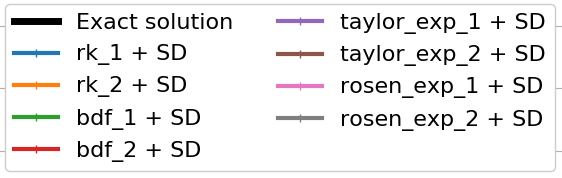
\includegraphics[width=0.5\textwidth]{images/resultats/legend.png}
    \caption{Légende des graphes des résultats}
    \label{fig:legend}
\end{figure}

\paragraph{}
Les graphes présentés dans cette partie utilisent la légende présentée en figure \ref{fig:legend}.


\subsection{Équation différentielles ordinaires}

    \paragraph{}
    Tout d'abord, nous avons regardé les différentes méthodes temporelles sur des EDO, afin de les étudier plus facilement et de manière plus exhaustive (c'est à dire sur plus de problèmes).

    \subsubsection{Cas linéaire}
        \paragraph{}
        Premièrement, nous allons nous intéresser à l'équation harmonique :
        \begin{equation}
            \left\{
            \begin{aligned}
                &\ddot{y} + y = 0 \\
                &\left(y, \dot{y}\right)_{t = 0} = \left(1, 0\right)
            \end{aligned}
            \right.
            \Longleftrightarrow
            \left\{
            \begin{aligned}
                &\dot{Y} = \begin{bmatrix}0 & 1\\-1 & 0\end{bmatrix}Y \\
                &Y_{t = 0} = \begin{pmatrix}1\\0\end{pmatrix}\\
                &Y = \begin{pmatrix}y\\\dot{y}\end{pmatrix}
            \end{aligned}
            \right.
            \label{eq:edo_harmonique}
        \end{equation}
        La solution de cette équation est la fonction cosinus.
        \begin{figure}[h!]
            \centering
            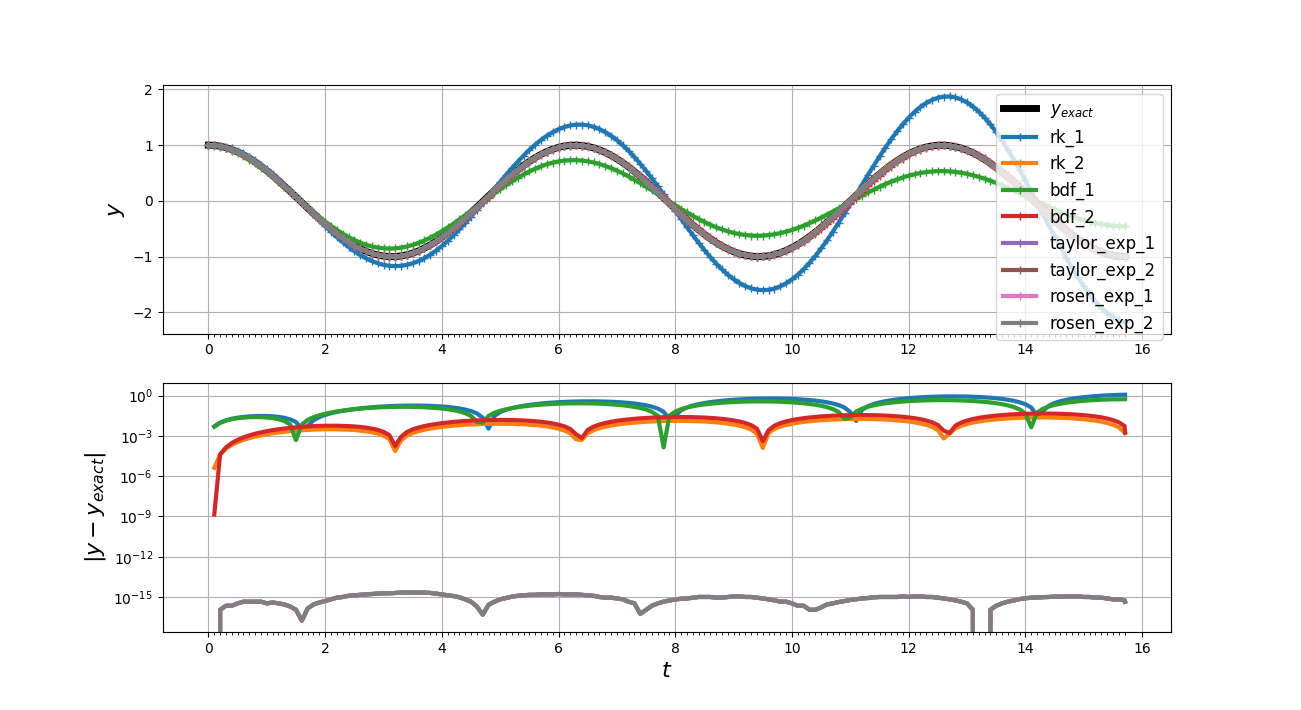
\includegraphics[width=\textwidth]{images/resultats/edo_sine.png}
            \caption{Résultats pour l'équation \ref{eq:edo_harmonique}, avec $\Delta t = 0.1$}
            \label{fig:edo_harmonique}
        \end{figure}

        \paragraph{}
        Sur la figure \ref{fig:edo_harmonique}, on voit les différents résultats calculés par les deux premiers ordres de chacune des méthodes (RK, BDF, exponentielles de Taylor et de Rosenbrock). La figure du haut représente la solution calculée en fonction du temps, et celle du bas l'écart à la solution théorique, en échelle semi-log. Nous pouvons y faire plusieurs observations :
        \begin{itemize}
            \item les courbes des différentes méthodes exponentielles sont toutes confondues
            \item les premiers ordres des méthodes RK et BDF s'éloignent de la solution exacte, en divergeant pour la méthode RK1 et en tendant vers 0 pour la méthode BDF1
            \item toutes les autres solutions calculées semblent confondues avec la solution théorique, y compris les premiers ordres des méthodes exponentielles
            \item en regardant le graphe du bas, on voit que l'erreur des méthodes RK2 et BDF2 sont du même ordre de grandeur, plus bas que celle des ordres 1 correspondants mais bien supérieurs à l'erreur des méthodes exponentielles, tout ordre confondu
        \end{itemize}

        \paragraph{}
        En regardant bien les équations, on se rend compte que, puisque cette équation à un second membre linéaire, une méthode exponentielle est censée calculer la solution exacte, inconditionnellement. Ainsi, nous avons résolu la même équation, mais avec un pas de temps bien supérieur. Le résultat de cette simulation est représenté sur la figure \ref{fig:edo_harmonique_2}. Cette fois, on ne voit plus les méthodes RK, qui divergent rapidement vers l'infini. On peut vérifier le constat précédent : alors que les méthodes BDF s'écrasent vers 0, les méthodes exponentielles, qui sont à nouveau confondues sur le graphe, calculent la solution presque exactement. La faible erreur que l'on observe est introduite par les calculs matriciels intervenant dans les méthodes exponentielles, et non par des erreurs de la méthode.
        \begin{figure}[H]
            \centering
            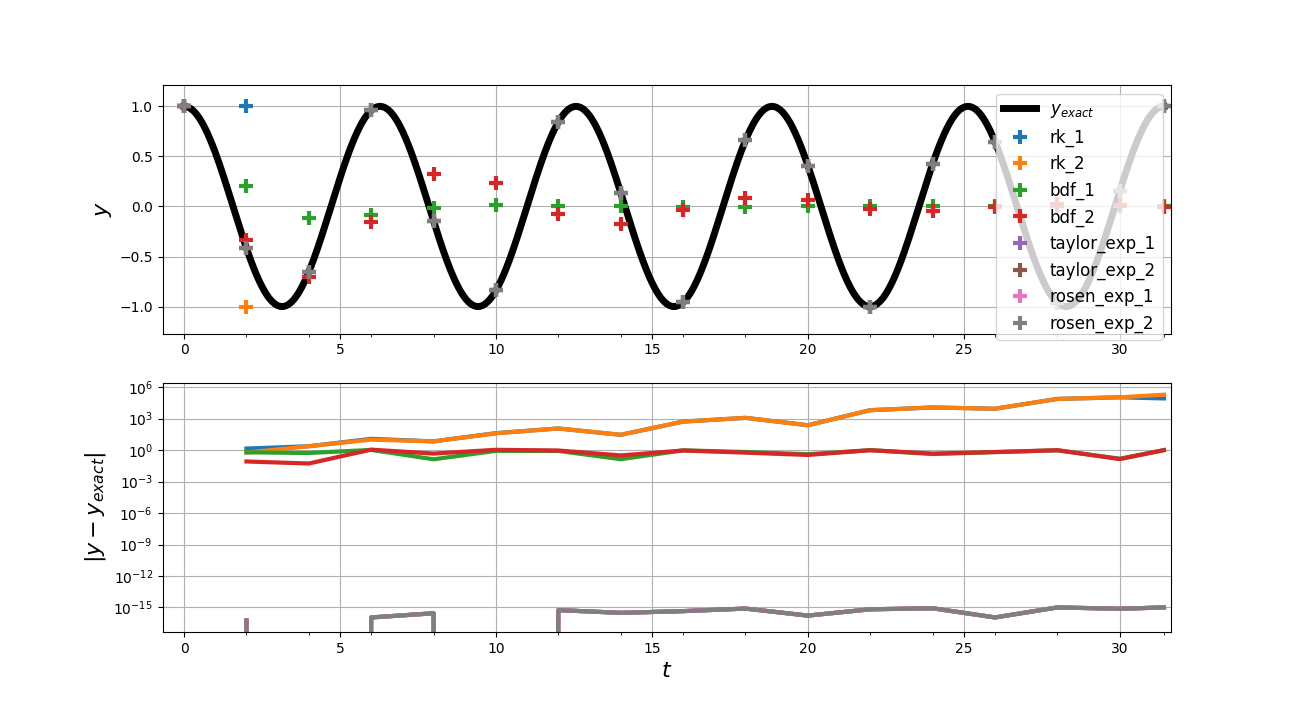
\includegraphics[trim = 0cm 0cm 0cm 1cm, clip, width=\textwidth]{images/resultats/edo_sine_large_dt.png}
            \caption{Résultats pour l'équation \ref{eq:edo_harmonique}, avec $\Delta t = 2$}
            \label{fig:edo_harmonique_2}
        \end{figure}

    \subsubsection{Cas raide}
        \paragraph{}
        Le deuxième cas que nous présentons ici est un cas non linéaire, dit \emph{raide}, présenté dans l'article \cite{stiff_equation}.
        L'équation résolue est :
        \begin{equation}
            \begin{split}
                \left\{
                \begin{aligned}
                    &\dot{y} = -50\left(y - \cos\left(t\right)\right) \\
                    &y\left(0\right) = 0
                \end{aligned}
                \right.
            \end{split}
        \label{eq:raide}
        \end{equation}
        Cette équation admet pour solution $y\left(t\right) = \frac{50}{2501}\sin\left(t\right)+\frac{2500}{2501}\cos\left(t\right) -\frac{2500}{2501}e^{-50t}$.
        \begin{figure}[H]
            \centering
            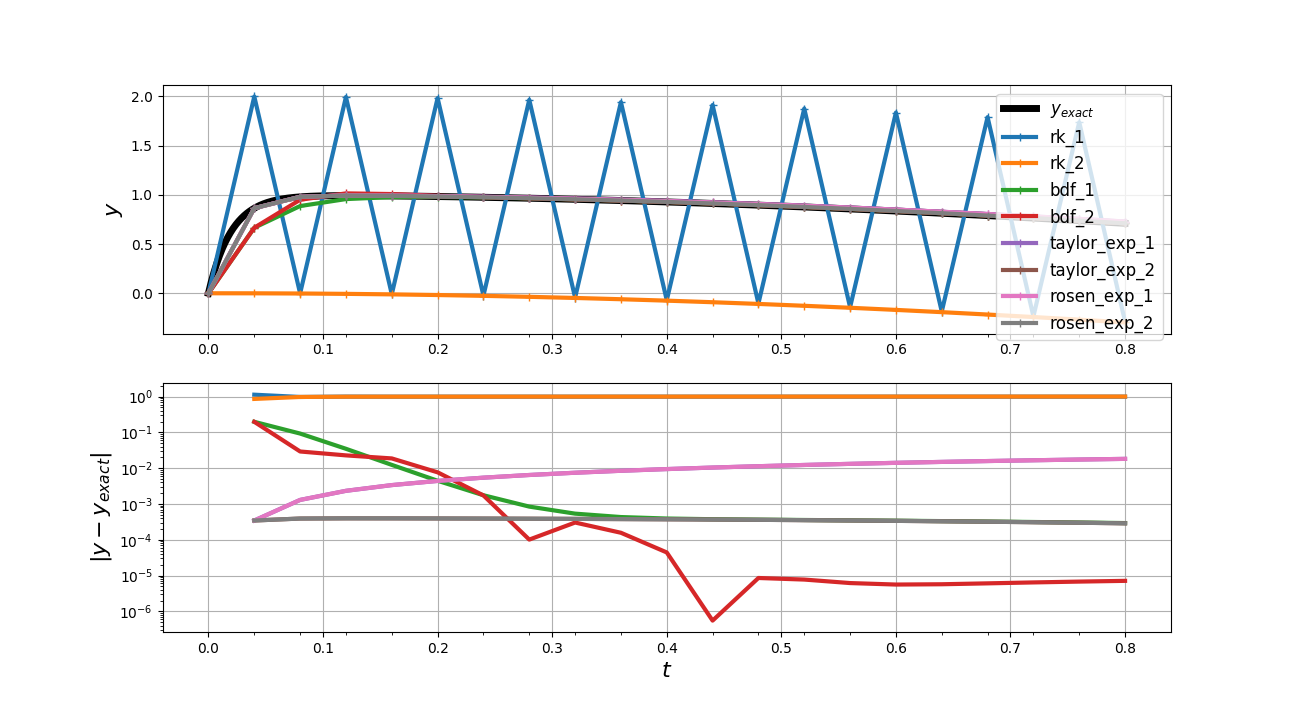
\includegraphics[trim = 0cm 0cm 0cm 1cm, clip, width=\textwidth]{images/resultats/edo_raide.png}
            \caption{Résultats pour l'équation \ref{eq:raide}, avec $\Delta t = 0.04$}
            \label{fig:edo_raide}
        \end{figure}

        \paragraph{}
        Sur la figure \ref{fig:edo_raide}, on voit à nouveau la solution calculée par les différentes méthodes, ainsi que l'écart à la solution analytique. On y fait les observations suivantes :
        \begin{itemize}
            \item les courbes des méthodes exponentielles de même ordre sont à nouveau confondues
            \item les méthodes explicites (RK) ne parviennent pas à évaluer une solution correcte avec un tel pas de temps, alors que les méthodes implicites (BDF) et exponentielles y arrivent
            \item les méthodes exponentielles d'ordre 2 sont plus précises que celles d'ordre 1, car elles prennent en compte le coté non autonome (la dépendance explicite en $t$) de l'équation \ref{eq:raide}.
        \end{itemize}

        \paragraph{}
        Grâce à ce cas, on peut donc voir que les méthodes exponentielles permettent aussi de résoudre des problèmes non linéaires, et même raides.

    \subsubsection{Cas non linéaire}
        \paragraph{}
        L'équation résolue ici est :
        \begin{equation}
            \begin{split}
                \left\{
                \begin{aligned}
                    &\dot{y} = y^2 \\
                    &y\left(0\right) = 0.1
                \end{aligned}
                \right.
            \end{split}
        \label{eq:nonlinear}
        \end{equation}
        Cette équation admet pour solution $y\left(t\right) = \frac{0.1}{1 - 0.1t}$. Sa particularité réside dans le fait qu'elle est fortement non linéaire, et diverge en un temps fini (ici $t = 10$). Pour l'étudier, on utilise une discrétisation temporelle irrégulière : on va réduire le pas de temps à mesure qu'on s'approche de la divergence pour mieux calculer la solution. La discrétisation utilisée ici est $t_{0\leq i\leq 19} = 10\left(1 - 10^{-i/19}\right)$.
        \begin{figure}[H]
            \centering
            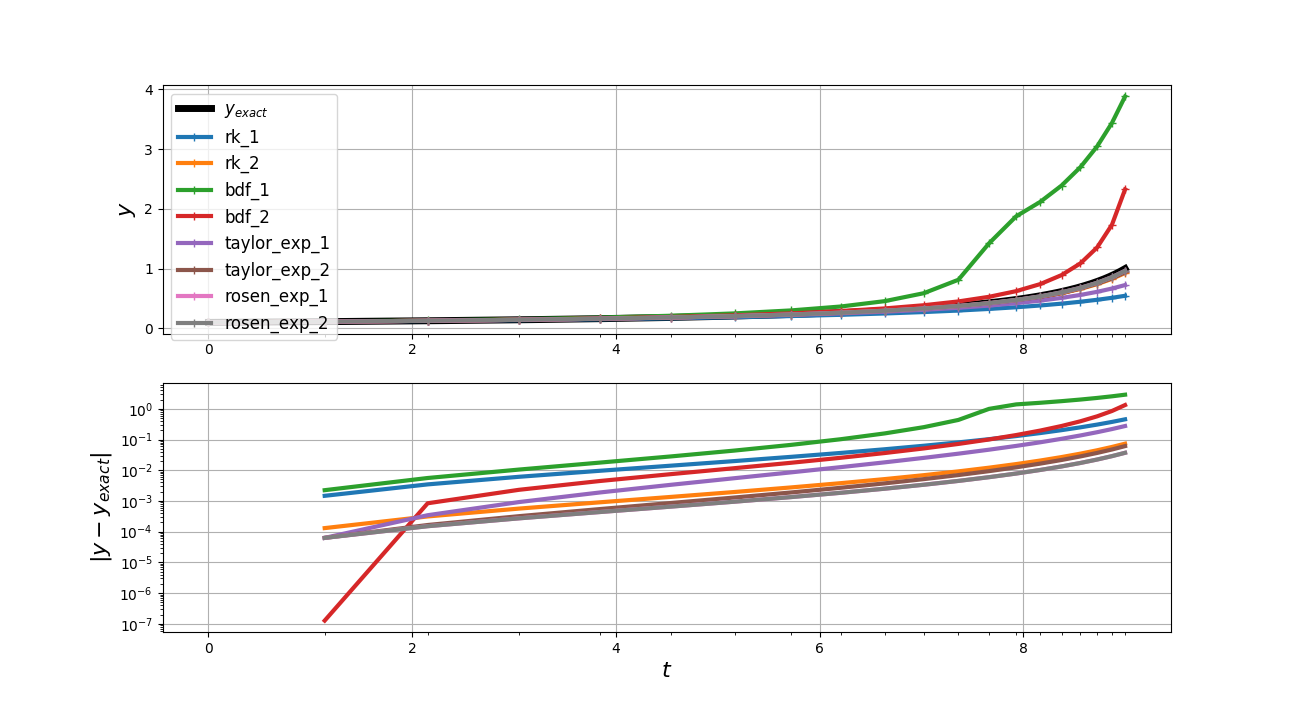
\includegraphics[trim = 0cm 0cm 0cm 1cm, clip, width=\textwidth]{images/resultats/edo_nonlinear.png}
            \caption{Résultats pour l'équation \ref{eq:nonlinear}, calculée aux instants $t_{0\leq i\leq 19} = 10\left(1 - 10^{-i/19}\right)$}
            \label{fig:edo_non_lineaire}
        \end{figure}

        \paragraph{}
        Sur la figure \ref{fig:edo_non_lineaire}, on affiche les résultats obtenus avec les mêmes méthodes que précédemment. On y observe les résultats suivants :
        \begin{itemize}
            \item cette fois-ci ce sont les méthodes BDF qui s'écartent beaucoup de la solution
            \item on a toujours que la précision augmente avec l'ordre de la méthode
            \item les méthodes de Rosenbrock sont meilleures que les méthodes de Taylor classiques, puisqu'elles actualisent la partie linéaire qu'elles prennent en compte à chaque pas de calcul
            \item puisque la partie linéaire prise en compte par les méthodes de Taylor classique reste la même le long du calcul et s'éloigne de la réelle partie linéaire de la solution, ces méthodes tendent vers les méthodes RK du même ordre (sur le graphe des erreurs, la courbe violette tend vers la bleue, et la marron tend vers la orange)
            \item les deux méthodes de Rosenbrock restent équivalentes, puisque la non linéarité est elle %linéaire
            autonome et n'évolue pas avec le temps (la hessienne du membre de droite est constante)
        \end{itemize}

        \paragraph{}
        Cette fois encore, les méthodes exponentielles restent meilleures que les autres méthodes du même ordre.

        \paragraph{}
        Finalement, ces cas tests sur des EDO ont permis de montrer que les méthodes exponentielles sont performantes à la fois sur les domaines d'utilisation des méthodes explicite, et aussi sur ceux des méthodes implicites. Et dans le meilleur des cas, le cas linéaire, elles permettent de résoudre exactement le problème donné.

\subsection{Équation aux dérivées partielles}

    \paragraph{}
    L'étude préliminaire avec des EDO permet de mieux comprendre les méthodes exponentielles, mais l'intérêt du client se porte sur les EDP. Pour tester les méthodes temporelles sur des EDP, nous utilisons un schéma spatial de Différences Spectrales (SD) d'ordre 2 en 1D, sur un intervalle avec des conditions aux limites périodiques.

    \subsubsection{Problème d'advection - diffusion}
        \paragraph{}
        Tout d'abord, le problème étudié est celui de l'advection - diffusion :
        \begin{equation}
            \frac{\partial y}{\partial t} + c\frac{\partial y}{\partial x} = d\frac{\partial^2 y}{\partial^2 x}
            \Longleftrightarrow \frac{\partial y}{\partial t} + \frac{\partial}{\partial x}\left(cy - d\frac{\partial y}{\partial x}\right) = 0
            \label{eq:edp_advection_diffusion}
        \end{equation}
        avec les paramètres $c$ et $d$ constants, et $d \ge 0$.
        \begin{figure}[H]
            \centering
            \begin{subfigure}{.5\textwidth}
                \centering
                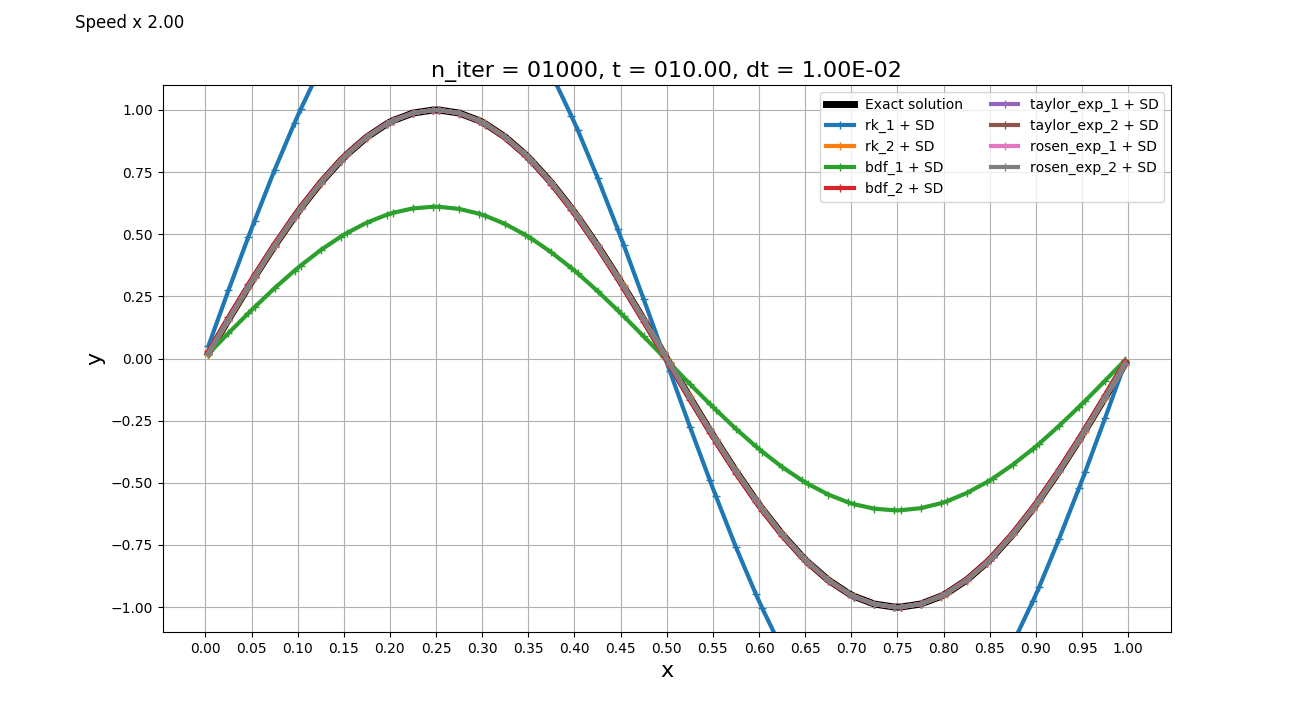
\includegraphics[trim = 0cm 0cm 1cm 1cm, clip, width=\textwidth]{images/resultats/edp_advection_1.png}
                \caption{t = 10}
                \label{fig:edp_advection_1}
            \end{subfigure}
            \begin{subfigure}{.5\textwidth}
                \centering
                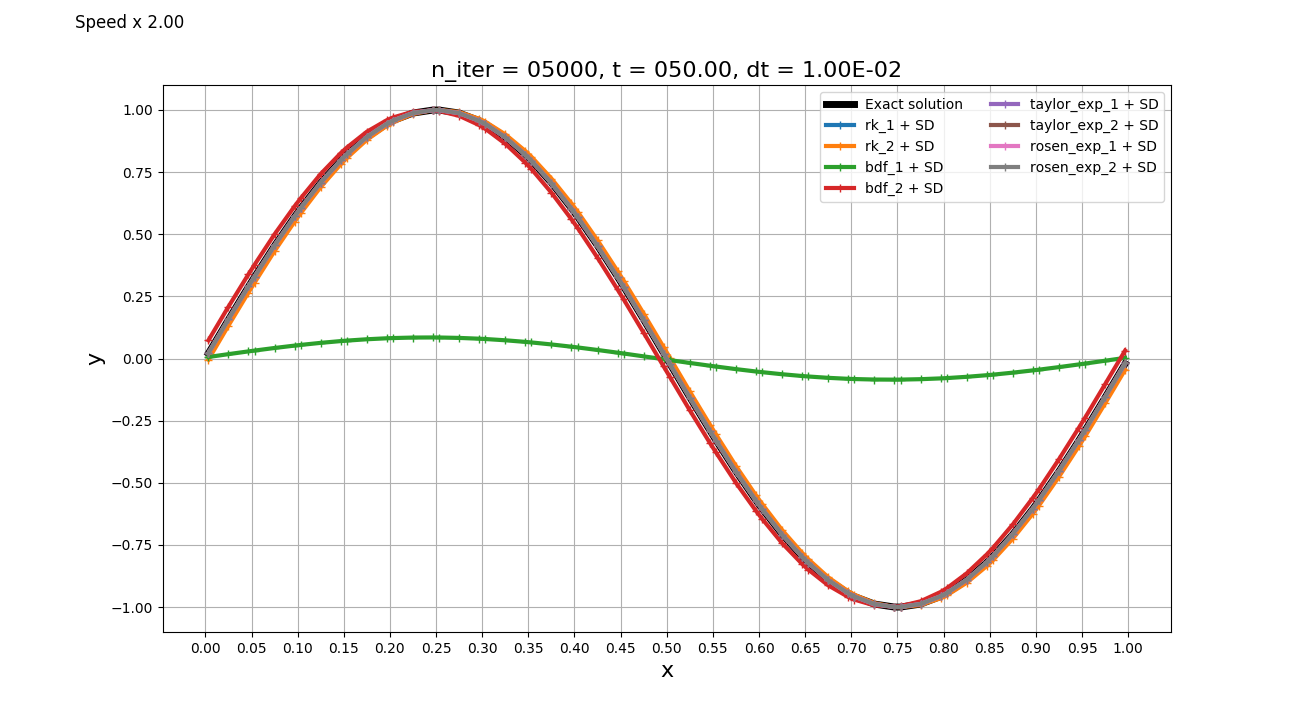
\includegraphics[trim = 0cm 0cm 1cm 0.5cm, clip, width=\textwidth]{images/resultats/edp_advection_2.png}
                \caption{t = 50}
                \label{fig:edp_advection_2}
            \end{subfigure}%
            \begin{subfigure}{.5\textwidth}
                \centering
                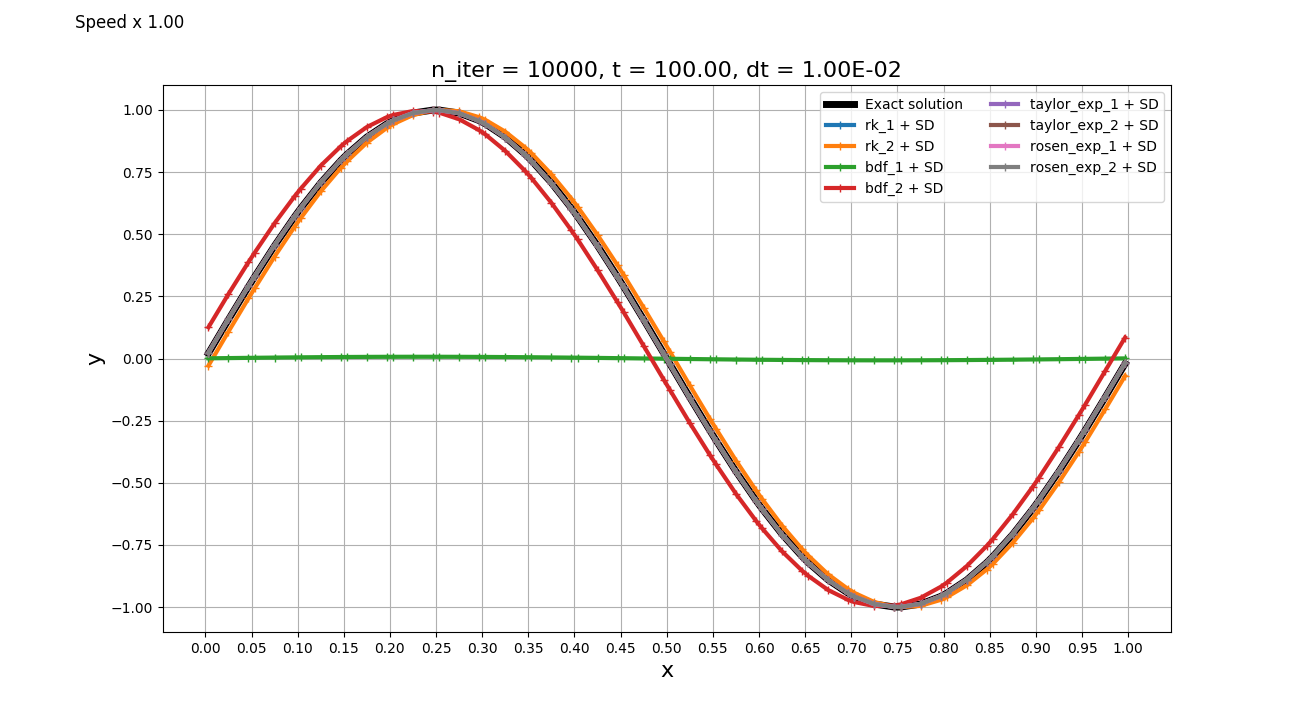
\includegraphics[trim = 0cm 0cm 1cm 0.5cm, clip, width=\textwidth]{images/resultats/edp_advection_3.png}
                \caption{t = 100}
                \label{fig:edp_advection_3}
            \end{subfigure}
            \caption{Solutions calculées pour le problème d'advection pure ($c = 0.5$, $d = 0$), avec un schéma spatial SD d'ordre 2 et un pas de temps $\Delta t = 0.01$ (CFL = 0.746)}
            \label{fig:edp_advection}
        \end{figure}

        \paragraph{}
        Tout d'abord, avec une équation d'advection pure ($c = 0.5$, $d = 0$), on regarde les résultats présentés sur la figure \ref{fig:edp_advection}.
        \begin{itemize}
            \item Sur la figure \ref{fig:edp_advection_1}, on voit qu'après 1000 itérations la méthode RK1 commence à diverger, et la méthode BDF1 à s'écraser vers 0.
            \item Sur la figure \ref{fig:edp_advection_2}, après 5000 itérations, la méthode BDF1 est très proche de 0, et on voit que les méthodes RK2 et BDF2 commencent à se séparer de la solution théorique.
            \item Sur la figure \ref{fig:edp_advection_3}, après 10000 itérations, les méthodes RK2 et BDF2 ont un déphasage bien visible par rapport à la solution théorique.
            \item Tout le long du calcul, les méthodes exponentielles sont indistinguables de la solution théorique.
        \end{itemize}
        \begin{figure}
            \centering
            \begin{subfigure}{.5\textwidth}
                \centering
                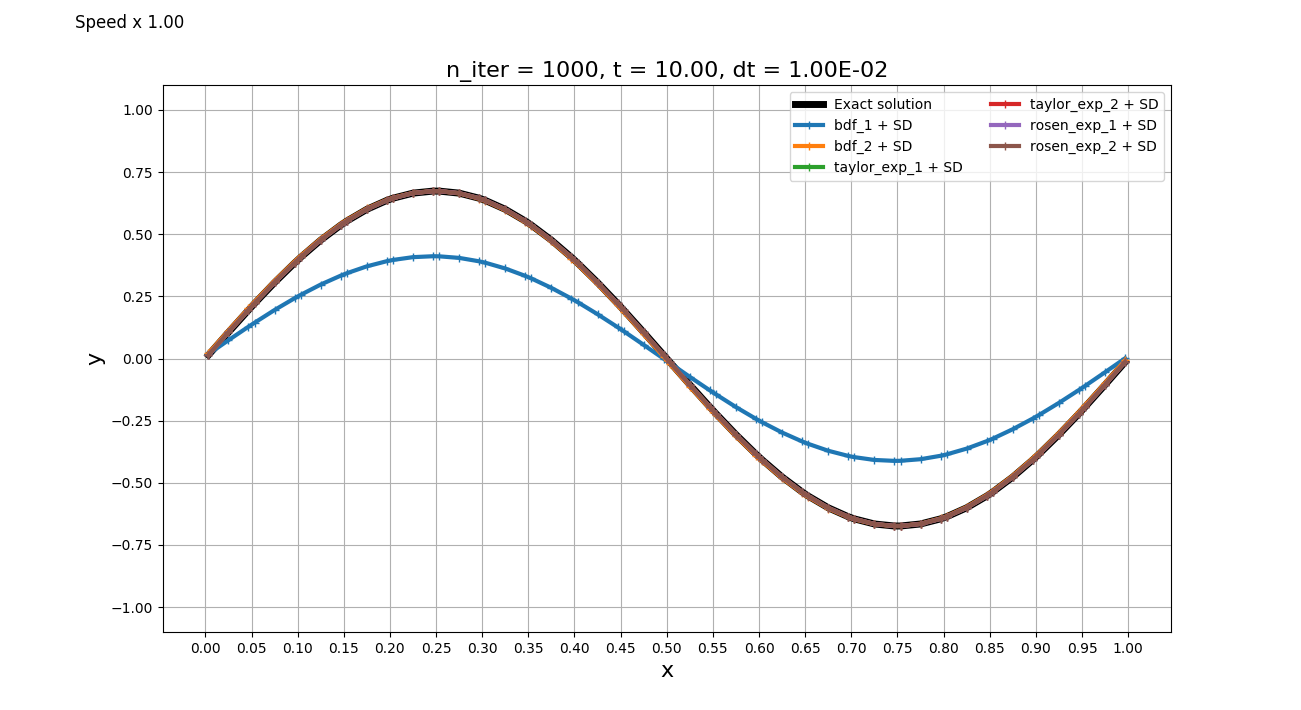
\includegraphics[width=\textwidth]{images/resultats/edp_adv_diff_cfl_1.png}
                \caption{$\Delta t = 0.01$ (CFL = 0.746)}
                \label{fig:edp_adv_diff_cfl_1}
            \end{subfigure}%
            \begin{subfigure}{.5\textwidth}
                \centering
                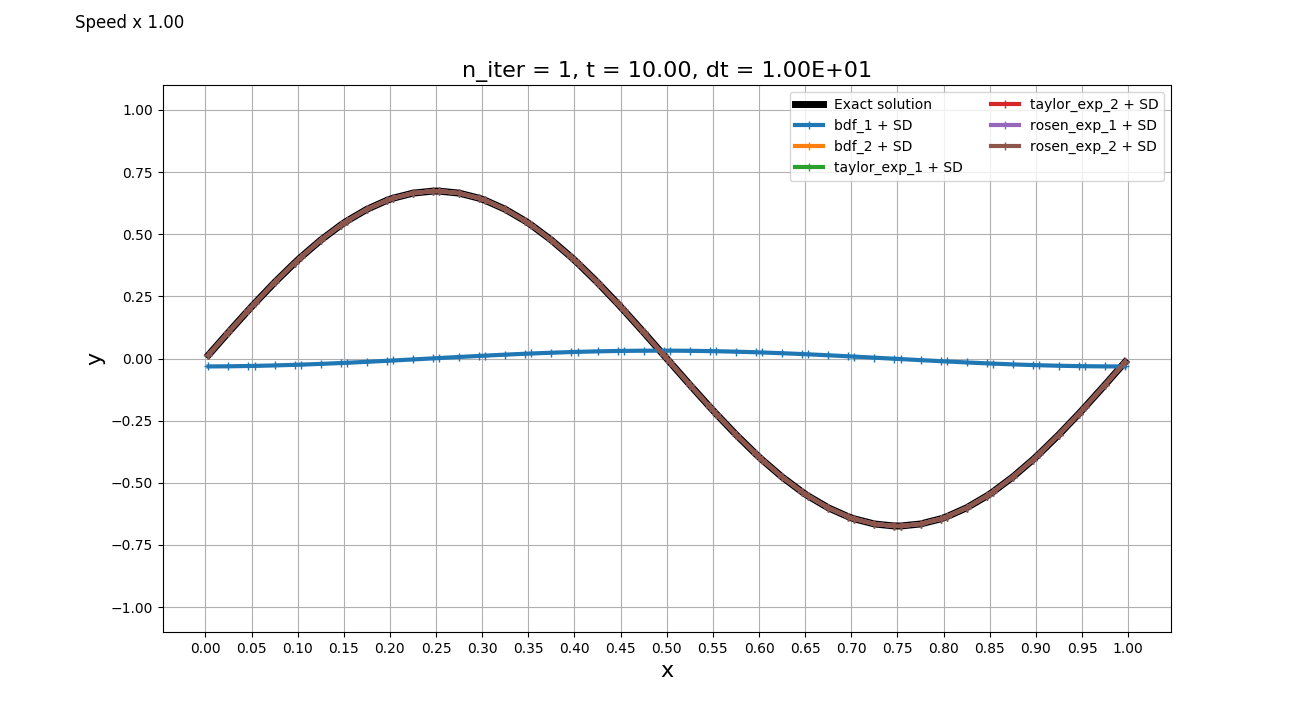
\includegraphics[width=\textwidth]{images/resultats/edp_adv_diff_cfl_2.png}
                \caption{$\Delta t = 10$ (CFL = 746.41)}
                \label{fig:edp_adv_diff_cfl_2}
            \end{subfigure}
            \caption{Solutions calculées pour le problème d'advection diffusion ($c = 0.5$, $d = 0.001$), avec un schéma spatial SD d'ordre 2, à t = 10 et pour différentes valeurs du pas de temps}
            \label{fig:edp_adv_diff_cfl}
        \end{figure}

        \paragraph{}
        Tout comme dans le cas de l'EDO linéaire vue précédemment, les méthodes exponentielles sont sensées résoudre ce problème d'advection de manière exacte, puisque la méthode SD donne un membre de droite linéaire pour des problèmes d'advection diffusion. Nous avons pu vérifier ceci grâce au cas présenté en figure \ref{fig:edp_adv_diff_cfl}. On y voit que :
        \begin{itemize}
            \item pour une faible valeur du nombre CFL la méthode BDF d'ordre 2 peut calculer une bonne approximation de la solution, sur la figure \ref{fig:edp_adv_diff_cfl_1}
            \item pour une plus grande valeur du nombre CFL la méthode BDF2 ne peut plus calculer d'approximation de la solution, sur la figure \ref{fig:edp_adv_diff_cfl_2}
            \item pour n'importe quel nombre de CFL arbitrairement grand, les méthodes exponentielles sont indistinguables de la solution théorique
        \end{itemize}

    \subsubsection{Équation de Burgers}
        \paragraph{}
        Les méthodes exponentielles résolvent ainsi très facilement les équations différentielles où le membre de droite est linéaire. Pour pouvoir conclure quant à leur performances, il faut d'abord les tester sur un problème non linéaire. Pour cela nous avons développé un code SD pour modéliser l'équation de Burgers :
        \begin{equation}
            \frac{\partial y}{\partial t} + y\frac{\partial y}{\partial x} = d\frac{\partial^2 y}{\partial^2 x}
            \Longleftrightarrow \frac{\partial y}{\partial t} + \frac{\partial}{\partial x}\left(\frac{y^2}{2} - d\frac{\partial y}{\partial x}\right) = 0
            \label{eq:burgers}
        \end{equation}
        \begin{figure}
            \centering
            \begin{subfigure}{.5\textwidth}
                \centering
                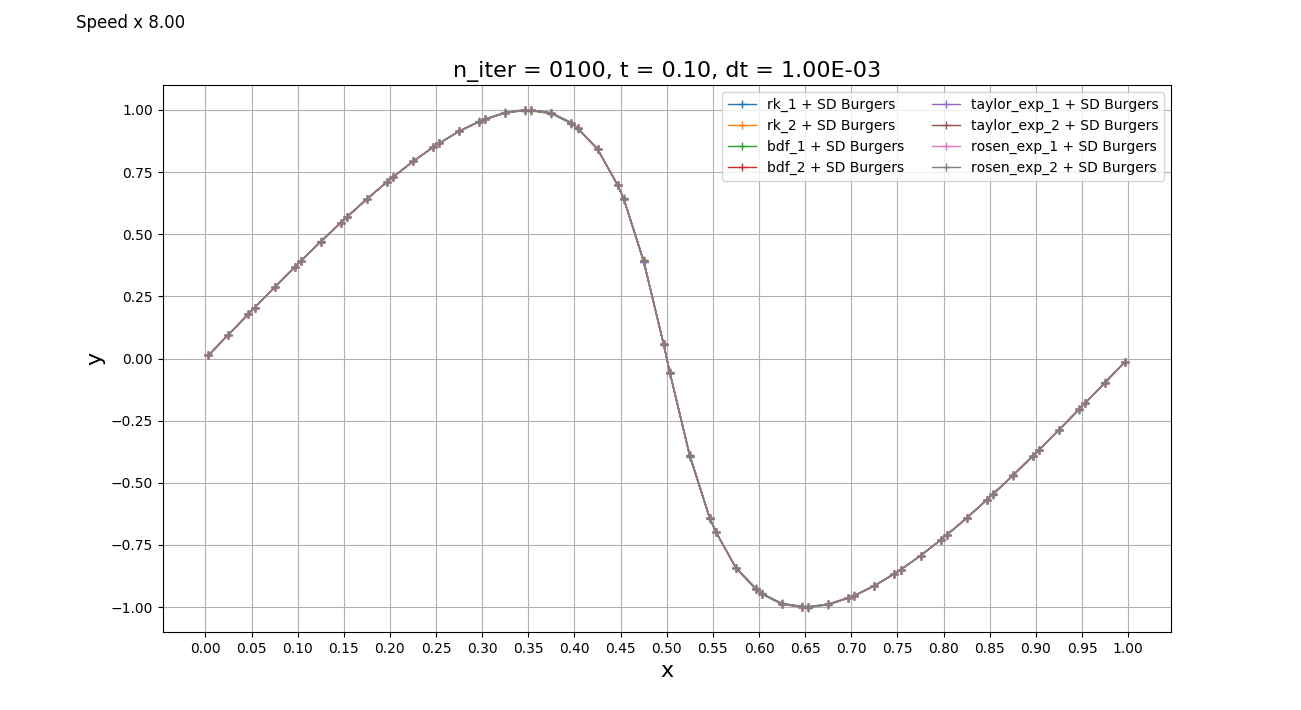
\includegraphics[width=\textwidth]{images/resultats/edp_burgers_1.png}
                \caption{t = 0.1}
                \label{fig:edp_burgers_1}
            \end{subfigure}%
            \begin{subfigure}{.5\textwidth}
                \centering
                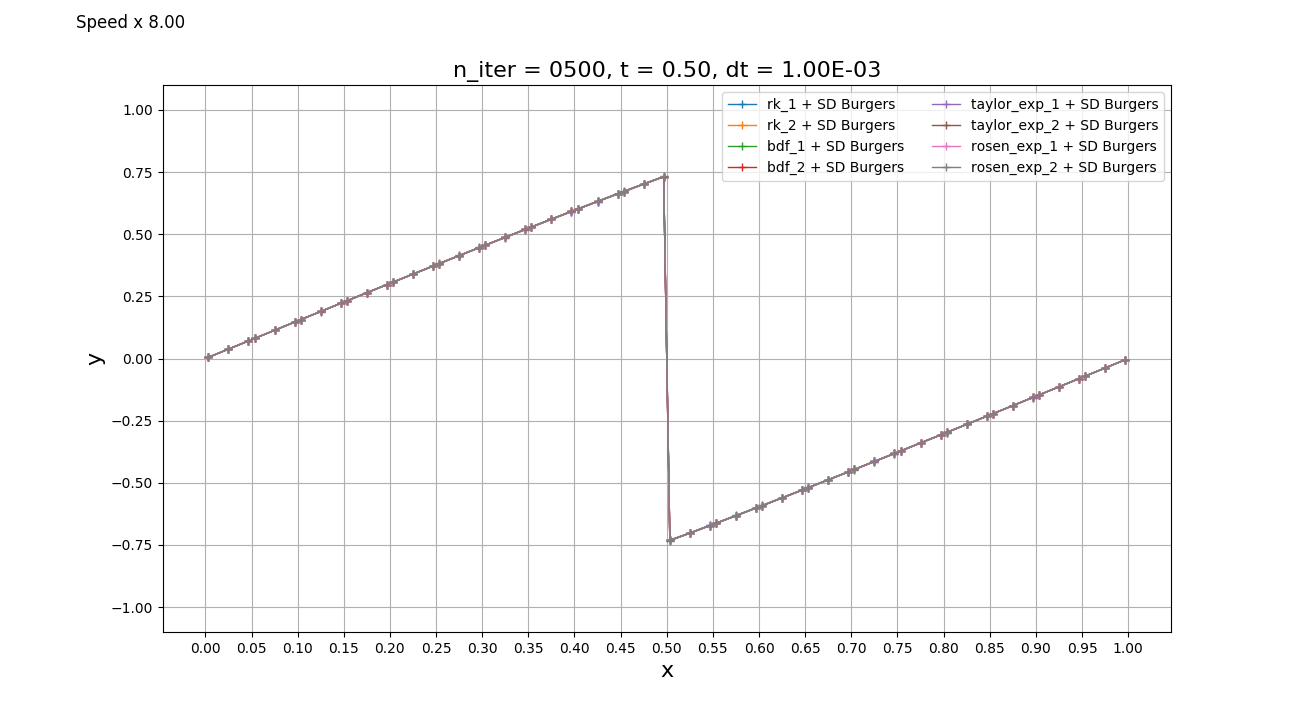
\includegraphics[width=\textwidth]{images/resultats/edp_burgers_2.png}
                \caption{t = 0.5}
                \label{fig:edp_burgers_2}
            \end{subfigure}
            \caption{Solutions calculées pour le l'équation de Burgers (equation \ref{eq:burgers}) non visqueuse ($d = 0$), avec un schéma spatial SD d'ordre 2, pour $\Delta t = 0.001$ (CFL = 0.149)}
            \label{fig:edp_burgers}
        \end{figure}

        \paragraph{}
        Sur la figure \ref{fig:edp_burgers}, on peut voir que les méthodes exponentielles donnent également des résultats satisfaisants sur des problèmes où le membre de droite n'est pas linéaire. En effet sur cette figure, toutes les courbes sont confondues. Il n'existe pas de solution analytique à l'équation \ref{eq:burgers} avec un sinus comme condition initiale sur un segment avec des conditions aux limites périodiques. Nous avons donc vérifié, avec des schémas connus, des pas de temps faibles et des maillages fins, que la solution affichée sur la figues \ref{fig:edp_burgers} est bien celle vers laquelle on tend (et c'est donc à priori la solution exacte). En étant confondues dans ces autres solutions convergées, les méthodes exponentielles nous montrent qu'elles peuvent résoudre cette équation de Burgers.

        \paragraph{}
        Il est cependant difficile de conclure quant aux performances des méthodes exponentielles pour résoudre cette équation, car le schéma des différences spectrales donne un second membre qui n'est pas continu, ce qui nous place en dehors du cadre d'application de la théorie présentée dans la partie précédente.


\subsection{Conclusion et perspectives}

    \paragraph{}
    Cette étude nous aura permis de mieux appréhender les méthodes exponentielles, en mettant en valeurs leurs atouts par rapport aux méthodes plus classiques de type RK et BDF. Grâce aux EDO, nous avons pu étudier toutes ces méthodes sur des cas très variés. Cette première démarche aura montré que les méthodes exponentielles possèdent les qualités de ces deux autres types de méthodes, et peuvent même, dans certains cas simples, résoudre exactement le problème. La conclusion pourrait être formulée de la manière suivante : \emph{dans le pire des cas c'est une méthode classique (RK ou BDF) et dans le meilleur des cas c'est une méthode exacte}.

    \paragraph{}
    La seconde partie de l'étude concerne les EDP. Nous avons montré que les méthodes exponentielles sont tout à fait applicables dans la résolution de ce type de problèmes. Toujours sur les problèmes qui ont un second membre linéaire, les méthodes exponentielles sont imbattables car elles permettent d'utiliser n'importe quel pas de temps, c'est à dire de déterminer n'importe quel état aussi loin dans le temps que voulu, en une seule itération.

    \paragraph{}
    Le plus grand défaut de ces méthodes temporelles reste leur coût de calcul : il est nécessaire de calculer des exponentielles de matrices, opération qui est très coûteuse d'un point de vue informatique. Pour contourner ce problème, nous nous sommes intéressés aux méthodes de Krylov, qui permettent d'accélérer énormément le calcul en offrant un compromis temps d'exécution - précision qui semble raisonnable.


\clearpage

\thispagestyle{empty}
\part*{Liste des sigles et acronymes}
\begin{acronym}
    \acro{PBS}{\emph{diagramme Product Breakdown Structure}}
    \acro{WBS}{\emph{diagramme Working Breakdown Structure}}
    \acro{RACI}{\emph{Réalisation, Approbation, Consultation, Information}}
    \acro{CFD}{\emph{Computational Fluid Dynamics (mécanique des fluides numérique)}}
    \acro{LES}{\emph{Large Eddies Simulation (simulation des grandes échelles de la turbulence)}}
    \acro{CFL}{\emph{condition de Courant–Friedrichs–Lewy}}
    \acro{SD}{\emph{Spectral Differences (différences spectrales)}}
    \acro{EDP}{\emph{Équation aux Dérivées Partielles}}
    \acro{EDO}{\emph{Équation Différentielle Ordinaire}}
    \acro{RK}{\emph{Runge - Kutta}}
    \acro{BDF}{\emph{Backward Differentiation Formula}}
\end{acronym}

\bibliography{biblio.bib}
\bibliographystyle{plain}

\begin{center}
    ISAE\\
    10, avenue Édouard Belin\\
    BP 54032\\
    31055 Toulouse CEDEX 4
\end{center}
\vspace*{\fill}

\end{document}

